%%%%%%%%%%%%%%%%%%%%%%%%%%%%%%%%%%%%%%%%%
% Programming/Coding Assignment
% LaTeX Template
%
% This template has been downloaded from:
% http://www.latextemplates.com
%
% Original author:
% Ted Pavlic (http://www.tedpavlic.com)
%
% Note:
% The \lipsum[#] commands throughout this template generate dummy text
% to fill the template out. These commands should all be removed when 
% writing assignment content.
%
% This template uses a Perl script as an example snippet of code, most other
% languages are also usable. Configure them in the "CODE INCLUSION 
% CONFIGURATION" section.
%
%%%%%%%%%%%%%%%%%%%%%%%%%%%%%%%%%%%%%%%%%

%----------------------------------------------------------------------------------------
%	PACKAGES AND OTHER DOCUMENT CONFIGURATIONS
%----------------------------------------------------------------------------------------

\documentclass{article}

\newtheorem{thm}{Theorem}
\usepackage{multirow}
\usepackage{amsthm}
\usepackage{amssymb}
\usepackage{url}
\usepackage{amsfonts}
\usepackage{algpseudocode}
\usepackage{mathtools}


\usepackage{fancyhdr} % Required for custom headers
\usepackage{lastpage} % Required to determine the last page for the footer
\usepackage{extramarks} % Required for headers and footers
\usepackage[usenames,dvipsnames]{color} % Required for custom colors
\usepackage{graphicx} % Required to insert images
\usepackage{listings} % Required for insertion of code
\usepackage{courier} % Required for the courier font
\usepackage{lipsum} % Used for inserting dummy 'Lorem ipsum' text into the template
\usepackage{url}
\usepackage{amsmath, amssymb} % cases and mathbb fix
\usepackage{xcolor}
\usepackage{hyperref}
\hypersetup{
    colorlinks,
    linkcolor={black},
    citecolor={blue!50!black},
    urlcolor={blue!80!black}
}
\newcommand{\quotes}[1]{``#1''}
% Margins
\topmargin=-0.45in
\evensidemargin=0in
\oddsidemargin=0in
\textwidth=6.5in
\textheight=9.0in
\headsep=0.25in
\def\kb{Ball-$k$-means}
\linespread{1.1} % Line spacing

% Set up the header and footer
\pagestyle{fancy}
\lhead{\hmwkAuthorName} % Top left header
\chead{\hmwkClass\ (\hmwkClassInstructor\ \hmwkClassTime) } % Top center head
\rhead{\firstxmark} % Top right header
\lfoot{\lastxmark} % Bottom left footer
\cfoot{} % Bottom center footer
\rfoot{Page\ \thepage\ of\ \protect\pageref{LastPage}} % Bottom right footer
\renewcommand\headrulewidth{0.4pt} % Size of the header rule
\renewcommand\footrulewidth{0.4pt} % Size of the footer rule

\setlength\parindent{0pt} % Removes all indentation from paragraphs

%----------------------------------------------------------------------------------------
%	CODE INCLUSION CONFIGURATION
%----------------------------------------------------------------------------------------

\definecolor{MyDarkGreen}{rgb}{0.0,0.4,0.0} % This is the color used for comments
\lstloadlanguages{R} % Load Perl syntax for listings, for a list of other languages supported see: ftp://ftp.tex.ac.uk/tex-archive/macros/latex/contrib/listings/listings.pdf
\lstset{language=R, % Use Perl in this example
        frame=single, % Single frame around code
        basicstyle=\small\ttfamily, % Use small true type font
        keywordstyle=[1]\color{Blue}\bf, % Perl functions bold and blue
        keywordstyle=[2]\color{Purple}, % Perl function arguments purple
        keywordstyle=[3]\color{Blue}\underbar, % Custom functions underlined and blue
        identifierstyle=, % Nothing special about identifiers                                         
        commentstyle=\usefont{T1}{pcr}{m}{sl}\color{MyDarkGreen}\small, % Comments small dark green courier font
        stringstyle=\color{Purple}, % Strings are purple
        showstringspaces=false, % Don't put marks in string spaces
        tabsize=5, % 5 spaces per tab
        %
        % Put standard Perl functions not included in the default language here
        morekeywords={},
        %
        % Put Perl function parameters here
        morekeywords=[2]{on, off, interp},
        %
        % Put user defined functions here
        morekeywords=[3]{test},
       	%
        morecomment=[l][\color{Blue}]{...}, % Line continuation (...) like blue comment
        numbers=left, % Line numbers on left
        firstnumber=1, % Line numbers start with line 1
        numberstyle=\tiny\color{Blue}, % Line numbers are blue and small
        stepnumber=5 % Line numbers go in steps of 5
}

% Creates a new command to include a perl script, the first parameter is the filename of the script (without .pl), the second parameter is the caption
\newcommand{\rscript}[2]{
\begin{itemize}
\item[]\lstinputlisting[caption=#2,label=#2]{#1.R}
\end{itemize}
}

%----------------------------------------------------------------------------------------
%	DOCUMENT STRUCTURE COMMANDS
%	Skip this unless you know what you're doing
%----------------------------------------------------------------------------------------

% Header and footer for when a page split occurs within a problem environment
\newcommand{\enterProblemHeader}[1]{
\nobreak\extramarks{#1}{#1 continued on next page\ldots}\nobreak
\nobreak\extramarks{#1 (continued)}{#1 continued on next page\ldots}\nobreak
}

% Header and footer for when a page split occurs between problem environments
\newcommand{\exitProblemHeader}[1]{
\nobreak\extramarks{#1 (continued)}{#1 continued on next page\ldots}\nobreak
\nobreak\extramarks{#1}{}\nobreak
}

\setcounter{secnumdepth}{0} % Removes default section numbers
\newcounter{homeworkProblemCounter} % Creates a counter to keep track of the number of problems

\newcommand{\homeworkProblemName}{}
\newenvironment{homeworkProblem}[1][Problem \arabic{homeworkProblemCounter}]{ % Makes a new environment called homeworkProblem which takes 1 argument (custom name) but the default is "Problem #"
\stepcounter{homeworkProblemCounter} % Increase counter for number of problems
\renewcommand{\homeworkProblemName}{#1} % Assign \homeworkProblemName the name of the problem
\section{\homeworkProblemName} % Make a section in the document with the custom problem count
\enterProblemHeader{\homeworkProblemName} % Header and footer within the environment
}{
\exitProblemHeader{\homeworkProblemName} % Header and footer after the environment
}

\newcommand{\problemAnswer}[1]{ % Defines the problem answer command with the content as the only argument
\noindent\framebox[\columnwidth][c]{\begin{minipage}{0.98\columnwidth}#1\end{minipage}} % Makes the box around the problem answer and puts the content inside
}

\newcommand{\homeworkSectionName}{}
\newenvironment{homeworkSection}[1]{ % New environment for sections within homework problems, takes 1 argument - the name of the section
\renewcommand{\homeworkSectionName}{#1} % Assign \homeworkSectionName to the name of the section from the environment argument
\subsection{\homeworkSectionName} % Make a subsection with the custom name of the subsection
\enterProblemHeader{\homeworkProblemName\ [\homeworkSectionName]} % Header and footer within the environment
}{
\enterProblemHeader{\homeworkProblemName} % Header and footer after the environment
}

%----------------------------------------------------------------------------------------
%	NAME AND CLASS SECTION
%----------------------------------------------------------------------------------------

\newcommand{\hmwkTitle}{Homework\ \#4} % Assignment title
\newcommand{\hmwkDueDate}{Thursday, March 2,  2023, 08:00 p.m.}% Due date
\newcommand{\hmwkClass}{B565-Data Mining\\} % Course/class
\newcommand{\hmwkClassTime}{} % Class/lecture time
\newcommand{\hmwkClassInstructor}{Instructor: Dr. H. Kurban, Head TA: Md R. Kabir} % Teacher/lecturer
\newcommand{\hmwkAuthorName}{Jash Shah} % Your name

%----------------------------------------------------------------------------------------
%	TITLE PAGE
%----------------------------------------------------------------------------------------

\title{
\vspace{2in}
\textmd{\textbf{\hmwkClass\ \hmwkTitle}}\\
\normalsize\vspace{0.1in}\small{Due\ on\ \hmwkDueDate}\\
\vspace{0.1in}\large{\textit{\hmwkClassInstructor\ }}
\vspace{3in}
}

\author{\textbf{\hmwkAuthorName}}
\date{\today} % Insert date here if you want it to appear below your name

%----------------------------------------------------------------------------------------

\begin{document}


\maketitle

%----------------------------------------------------------------------------------------
%	TABLE OF CONTENTS
%----------------------------------------------------------------------------------------

%\setcounter{tocdepth}{1} % Uncomment this line if you don't want subsections listed in the ToC

\newpage





\section*{ $k$-means Algorithm in Theory}
This part is provided to help you implement $k$-means clustering algorithm.

{\small
\begin{center}
\begin{algorithmic}[1]\label{kmeans}
\State{\bf ALGORITHM} \texttt{k-means}
\State {\bf INPUT} (\textsf{data} $\Delta$, distance $d:\Delta^2\rightarrow \mathbb{R}_{\geq 0}$, \textsf{centoid number} $k$, \textsf{threshold} $\tau$)
\State {\bf OUTPUT} (\textsf{Set of centoids} $\{c_1, c_2, \ldots, c_k\}$)
\State
\State \texttt{***} $Dom(\Delta)$ denotes domain of data.
\State
\State \texttt{***} Assume centroid is structure $c = (v \in DOM(\Delta), B\subseteq \Delta)$
\State  \texttt{***} $c.v$ is the centroid value and $c.B$ is the set of nearest points.
\State \texttt{***}  $c^{i}$ means centroid at $i^{th}$ iteration. 
\State
\State $i = 0$
\State \texttt{***} Initialize Centroids
\For{$j = 1,k$}
\State $c_j^i.v \gets  random(Dom(\Delta))$
\State $c_j^i.B \gets \emptyset$
\EndFor
\State
\Repeat
\State $i \gets i + 1$
\State \texttt{***} Assign data point to {\it nearest} centroid
\For {$\delta \in \Delta$}
\State $c_j^i.B \gets c.B \cup \{\delta\}$, where $\min_{c_j^i}\{d(\delta, c_j^i.v)\}$
\EndFor
\For {$j = 1, k$}
\State \texttt{***} Get size of centroid
\State $n \gets |c_j^i.B|$
\State \texttt{***} Update centroid with average 
\State $c_j^i.v \gets (1/n)\sum_{\delta \in c_j^i.B} \delta$
\State \texttt{***} Remove data from centroid
\State $c_j^i.B \gets \emptyset$
\EndFor
\State \texttt{***} Calculate scalar product (abuse notation and structure slightly)
\State \texttt{***} See notes
\Until{$((1/k)\sum_{j=1}^k~|| c^{i-1}_j-c^{i}_j||) < \tau$}
\State {\bf return} ($\{c_1^i, c_2^i, \ldots, c_k^i\}$) 
\end{algorithmic}
\end{center}}
\subsection*{$k$-means on a tiny data set.}
Here are the inputs:
\begin{eqnarray}
\Delta &=& \{  (2, 5),  (1,5) , (22, 55), (42, 12), (15,16)\}\\
d((x_1, y_1) ,(x_2, y_2)) &=& [(x_1-x_2)^2 + (y_1 - y_2)^2)]^{1/2}\\
k &=&2\\
\tau &=& 10
\end{eqnarray}

Observe that $Dom(\Delta) = \mathbb{R}^2$.  We now work through $k$-means. We ignore the uninformative assignments.  We remind the reader that $\mathsf{T}$ means transpose.

\begin{center}
\begin{algorithmic}[1]
\State $i \gets 0$
\State \texttt{***} Randomly assign value to first centroid.
\State $c^0_1.v \gets random(Dom(\Delta)) = (16,19)$
\State \texttt{***} Randomly assign value to second centroid.
\State $c^0_2.v \gets random(Dom(\Delta)) = (2,5)$
\State $i \gets i + 1$
\State \texttt{***} Associate each datum with nearest centroid
\State $c^1_1.B = \{(22, 55), (42, 12), (15,16)\}$
\State $c^1_2.B = \{(2,5), (1,5)\}$
\State \texttt{***} Update centroids
\State $c^1_1.v \gets (26.3, 27.7) = (1/3)((22,55) + (42,12) + (15,16))$
\State $c^1_2.v \gets (1.5, 5) = (1/2)((2,5) + (1,5))$
\State \texttt{***} The convergence condition is split over the next few lines to explicitly show the calculations
\State $(1/k)\sum_{j=1}^k~|| c^{i-1}_j-c^{i}_j|| = (1/2)(||c^0_1 - c^1_1||+ ||c^0_2 - c^1_2||) = (1/2) (||{2 \choose 5} - {1.5 \choose 5}|| + ||{16 \choose 19} - {26.3 \choose 27.7}||)$
\State $ = (1/2)[({.5 \choose 0}^{\mathsf{T}}{.5 \choose 0})^{(1/2)} + ({-9.7 \choose  -8.7}^{\mathsf{T}}{-9.7 \choose  -8.7})^{(1/2)})] = (1/2)(\sqrt{.5} + \sqrt{169.7}) \sim (1/2)(13.7) = 6.9$
\State Since the threshold is met $(6.9 < 10)$, $k$-means stops, returning $\{(26.3, 27.7), (1.5,5)\}$
\end{algorithmic}
\end{center}

\newpage
%----------------------------------------------------------------------------------------
%	PROBLEM 1
%----------------------------------------------------------------------------------------

\begin{homeworkProblem}
For this problem we are going to use a diabetes data set collected from many US hospitals on the purpose of analyzing the factors causing readmission  of diabetic patients. You can download the data from here \href{https://archive.ics.uci.edu/ml/datasets/Diabetes+130-US+hospitals+for+years+1999-2008}{[link]}. The web-page comes with a downloadable link along with the description of the data.

Answer the following questions [\textbf{20 points}]:
\begin{enumerate}
\item Briefly describe this data set--what is its purpose?  How should it be used? What are the kinds of data it's using?

   \subsection{Discussion of  data} 
   Answer here$\ldots$
   \begin{itemize}
    \item The Diabetes Dataset of 130 US Hospitals is a dataset repository of medical records documenting hospitalizations of diabetic patients across 130 hospitals in the United States between 1999 and 2008. 
    \item With over 100,000 records, the dataset comprises 50 variables that capture a range of patient demographics, medical history, medications, and clinical measurements.
    \item The Dataset also contains various drugs administered to the patients
    \item The dataset's primary objective is to examine the factors that contribute to readmission of diabetic patients.
    \item Readmitted is a class variable having values (NO,>30,<30) which indicates the number of days after discharge a patient is readmitted
    \item \textbf{Use of Dataset} 
    \\ The dataset is widely used in research on diabetes and healthcare outcomes, and has contributed to a better understanding of the factors that influence diabetes management and outcomes in the United States
    \item Based on specific requirement we can apply numerous Data Mining tasks such as classification based on target variables, Perform Clustering to group the patients and help the doctors prioritize.
\end{itemize}
\item  Using \textit{R/Python}, show code that answers the following questions:
\begin{enumerate}
\item    How many entries are in the data set? 
\subsection{R/Python script }
\begin{lstlisting}[language=R]
# Sample R Script With Highlighting

\end{lstlisting}

\begin{lstlisting}[language=Python]
# Sample Python Script With Highlighting
import pandas as pd
import swifter
df= pd.read_csv('diabetic_data.csv')
df.shape
(101766, 50)
#The number of rows are 101766 and number of columns are 50
\end{lstlisting}
\begin{itemize}
    \item \textbf{The number of rows are 101766 and number of columns are 50}
\end{itemize}
\item  How many unknown or missing data are in the data set? 
\subsection{R/Python script }
\begin{lstlisting}[language=R]
# Sample R Script With Highlighting

\end{lstlisting}

\begin{lstlisting}[language=Python]
# Sample Python Script With Highlighting
df1=pd.DataFrame(df.isna().sum())
df1=df1.reset_index()
df1.columns=['Column_Names','Count_of_Nan_Values']
df2=df1[df1['Count_of_Nan_Values']!=0].
sort_values(by=['Count_of_Nan_Values'],ascending=False)
df2['Percentage_of_NAN']=df2['Count_of_Nan_Values']/len(df)*100
print('The Nan Value columns with percentage are as follows')
print(df2)
#Initially there are no Null values however 
when we replace #Question mark with Nan we 
get to see Null values
#Checking Null Values
import numpy as np
df.replace({'?':np.nan},inplace=True)
df1=pd.DataFrame(df.isna().sum())
df1=df1.reset_index()
df1.columns=['Column_Names','Count_of_Nan_Values']
df2=df1[df1['Count_of_Nan_Values']!=0]
.sort_values(by=['Count_of_Nan_Values'],ascending=False)
df2['Percentage_of_NAN']=df2['Count_of_Nan_Values']/len(df)*100
print('The Nan Value columns with percentage are as follows')
print(df2)
#Output
The Nan Value columns with percentage are as follows
         Column_Names  Count_of_Nan_Values  Percentage_of_NAN
5              weight                98569          96.858479
11  medical_specialty                49949          49.082208
10         payer_code                40256          39.557416
2                race                 2273           2.233555
20             diag_3                 1423           1.398306
19             diag_2                  358           0.351787
18             diag_1                   21           0.020636


\end{lstlisting}
\textbf{Thus we can see after applying transformation of replacing '?' with NAN we get columns [Weight,MedicalSpeciality,Payercode,Race,Diag3,Diag2,Diag1] as Null}
\\\textbf{The Percentage and values of Null is shown in the output above}
\item Create histograms for attributes \{\texttt{age}, \texttt{num\_lab\_procedures}, \texttt{num\_medications}\}. Label the plots properly. Discuss the distribution of values \textit{e.g.}, are uniform, skewed, normal.  Place images of these histograms into the document. Show the Python or R code that you used below and discussion below that. 
\subsection{R/Python script }
\begin{lstlisting}[language=R]
# Sample R Script With Highlighting

\end{lstlisting}

\begin{lstlisting}[language=Python]
# Sample Python Script With Highlighting
import matplotlib.pyplot as plt
import seaborn as sns
#Dropping columns with more than 40 percent null values
df.drop(['weight','payer_code','medical_specialty'],
axis=1,inplace=True)
#Changing the readmitted column
df['readmitted'] = df['readmitted'].replace({'>30':1,'<30':1,'NO':0})
#Replacing Age with mean
df['age'] = df['age'].replace({'[70-80)': 75, 
'[60-70)': 65, '[50-60)': 55, '[80-90)': 85,
'[40-50)': 45, '[30-40)': 35, '[90-100)': 95,
'[20-30)': 25, '[10-20)': 15, '[0-10)': 5})
sns.histplot(df['age'],kde=True,bins=10)
plt.title('Histogram with KDE of Age vs Frequency')
plt.xticks(rotation=90);
#Checking the distribution 
from scipy.stats import shapiro
#The Shapiro-Wilk test (often referred to as the Shapiro test) 
#is a statistical test used to assess 
whether a set of data follows a normal distribution
stat,p = shapiro(df['age'])
alpha = 0.05
#Checking the signiface value
if p > alpha:
    #The Null hypothesis is a distribution sample is Normally distributed
    print('Sample seems Gaussian (fail to reject H0)')
    #The Alternate hypothesis is a distribution is not normally distributed
else:
    print('Sample does not seems Gaussian (reject H0)')
#Sample does not seems Gaussian (reject H0)

#Checking Skewness test 
from scipy.stats import skewtest
#The skewtest is a statistical test that is used to assess
#whether a set of data is symmetric or skewed.
#The test is based on the comparison of the observed skewness 
#of data to the expected skewness under the assumption of normality. 
statistic, p_value = skewtest(df['age'])
alpha = 0.05
#Checking the significance value
if p_value > alpha:
    #Null hypothesis is data is not skewed
   print('Sample is symmetric (fail to reject H0)')
    #Alternate hypothesis is data is skewed
else:
   print('Sample is skewed (reject H0)')
#Sample is skewed (reject H0)

#Plotting  histogram of Number of lab procedures

sns.histplot(df['num_lab_procedures'],kde=True);
plt.title('Number_of_lab_procedures Histogram')
plt.show()

#Plotting Number of Medications
sns.histplot(df['num_medications'],kde=True)
plt.title('Number of medications histogram')
plt.show()
import numpy as np
import scipy.stats as stats
skewness = stats.skew(df['num_medications'])
#Check the Skwewness
print("Skewness:", skewness)
#Conditions with skewness and visual inspection
if skewness > 0:
    print("The distribution is normal distribution with right-tailed.")
else:
    print("The distribution is not right-tailed.")
Skewness: 1.3266525795561763
The distribution is normal distribution with right-tailed.



\end{lstlisting}

\subsection{Discussion of Findings}
Answer here$\ldots$
\begin{itemize}
    \item After plotting various graphs we can either check their distribution visually or by checking statistics test:
    \item Shapiro Wilk test is used to check Normality
    \item Skewtest is used for checking if data is skewed or Symmetric
    \item Chi Square test is to check Poisson Distribution
\end{itemize}
\begin{itemize}
    \item \textbf{Age is a skewed distribution}
    \item \textbf{Number of Lab pocedures is a skewed distribution and is bimodal}
    \item \textbf{Number of Medications is a normal distribution with right tail since the skwewness value is positive}
\end{itemize}


\subsection{Plots }
\begin{subfigure}
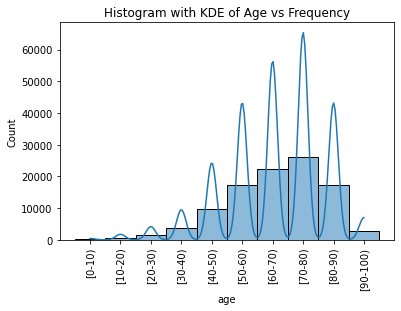
\includegraphics[width=0.5\columnwidth]{hw#4/1.png}
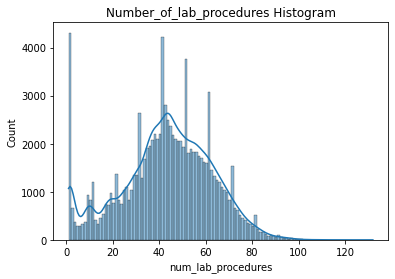
\includegraphics[width=0.5\columnwidth]{hw#4/2.png}
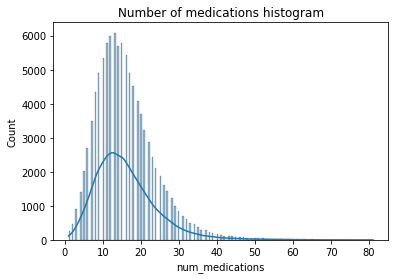
\includegraphics[width=0.5\columnwidth]{hw#4/3.png}
\end{subfigure}

\end{enumerate}

\item  Make a scatter plots 
of [\texttt{time\_in\_hospital}, 
\texttt{num\_medications}] 
and [\texttt{num\_medications}, 
\texttt{num\_lab\_procedures}] variables and color the data points with the class variable [\texttt{readmitted}]. Discuss the plots, i.e., do you observe any relationships between variables? Show the Python or R code that you used below and discussion below that.
\subsection{R/Python script }
\begin{lstlisting}[language=R]
# Sample R Script With Highlighting

\end{lstlisting}

\begin{lstlisting}[language=Python]
# Sample Python Script With Highlighting
sns.scatterplot(data=df, y='num_medications', x='time_in_hospital', 
hue='readmitted');
plt.title('Scatterplot of Num_Medications and Time_In_Hospital')
plt.show()
sns.scatterplot(data=df, x='num_medications', y='num_lab_procedures', 
hue='readmitted')
plt.title('Scatterplot of num_lab_procedures and num_medications')
plt.show()
df.corr()[['num_lab_procedures','num_medications']].
loc[['time_in_hospital','num_lab_procedures']]
 	num_lab_procedures 	num_medications
time_in_hospital 	0.31845 	0.466135
num_lab_procedures 	1.00000 	0.268161

\end{lstlisting}
\end{enumerate}
\end{enumerate}


\subsection{Discussion of Findings}
Answer here$\ldots$
\begin{itemize}
    \item \textbf{For Graph 1}
    \item In the first scatter plot, we can observe that there is a statistically positive relationship between time in hospital and num medications.
    \item The correlation between number of medications is \textbf{0.466}
    \item This indicates the more a patient stays in hospital more a patient has to take medicines.
    \item Additionally ,we can see that the readmitted variable does not seem to have a strong relationship with either variable.
    \item \textbf{For Graph 2}
    \item In the second scatter plot, we can observe that there is a weak positive relationship between num of medications and num of lab procedures. 
    \item The correlation between Num of medications and number of lab procedures is \textbf{0.2681}
     \item We can see that the readmitted variable does not seem to have a strong relationship with either variable.
    
\end{itemize}

\subsection{Plots }
\begin{subfigure}
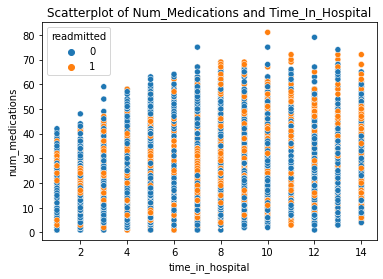
\includegraphics[width=0.5\columnwidth]{hw#4/4.png}
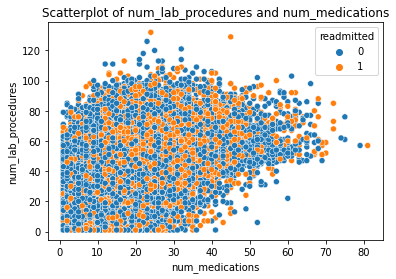
\includegraphics[width=0.5\columnwidth]{hw#4/5.png}

\end{subfigure}
\end{enumerate}

\end{homeworkProblem}

%----------------------------------------------------------------------------------------
%	PROBLEM 2
%----------------------------------------------------------------------------------------


\begin{homeworkProblem}

The pseudo-code for $k$-means and a running example of $k$-means on a small data set are provided above. Answer the following questions [\textbf{10 points}]:

\begin{enumerate}
  \item[2.1] Does $k$-means always converge? Given your answer, a bound on the iterate must be included. How is
its value determined?
\begin{itemize}
    \item From the above mentioned Algorithm, We can conclude that K means doesnt always converge to a global optimal solution,However given the covergence criteria K means is supposed to converge at a local minimum.
    \item K means may not converge due to the following reasons:
    \item \textbf{Initialization of centroids}: Since k means is a greedy algorithm it is extremely sensitive to the Initial Centroid selection.
    \\ If the centroids are not selected properly, K means may converge to suboptimal solution
    \item \textbf{Number of CLusters}: Although there are numerous methods to decide the number of clusters by elbow method,Dunn Index, Silheoutte Analysis,There is a possibility if number of clusters is set too high or too low, K means will comverge to a sub optimal solution
    \item \textbf{Outliers}: If the dataset contains outliers,
    K means will not converge as expected
    \item \textbf{Non Spherical Clusters}: The main assumption in K means is the Spherical nature of clusters with similar variaces, However K means will not converge optimally if the clusters are non spherical
    \item \textbf{Local Convergence} However, K means will, always converge to a local optimum as K means can be seen as an optimization problem and we can reduce the Sum of Squared errors within the clusters. Thus as any minima finding solution K means can guarantee a local optimum
\end{itemize}
\textbf{Bound on Iterate}
\begin{itemize}
    \item \textbf{Convergence Criteria} The above algorithm assumes a threshold value Tou which is the difference in magnitude of Old centroid Vector and New Centroids Vector.
    \item However we can also include a bound on iterate to avoid Infinite Loops, As in some cases there can be a situation the convergence criteria is never met and K means algorithm runs indefinitely
    \item By setting a bound on iterate we can also reduce the computational cost and have a trade off between accuracy and Computational Cost.
\end{itemize}
\textbf{Value of Bound on Iterate}
\begin{itemize}
    \item The above mentioned algorithm converges on Tou,and the value of Tou must be decided by looking at the clustering variables.
    \item By applying Domain Knowledge we can achieve a substantial value of Tou
    \item However, Since it is a greedy algorithm and the search space is infinite we have to do trial and error method and select the best Tou for Clusters.
    \item For the number of iterations we can plot a graph of convergence vs the number of iterations it takes to converge.
    \item This would give a fair idea on selecting the number of iterations,However due to the random nature of Cluster Initialization ,We can perform a trial and error method and start increasing the number of iterations starting from a low value.
    \item However for a huge dataset, We can set a bound roughly proportional to the computational cost. 
\end{itemize}
  \item[2.2] What is the run-time of this algorithm?
  \begin{itemize}
      \item The run time algorithm depends on number of factor such as initialization of centroids,number of clusters,The initialization method and convergence criterion.
      \item However the generalized run time depends on 
      \textbf{O(K*N*D)} where K is the Number of Clusters,N is the Number of datapoints and D is the dimensionality of data.
      \item With i number of iterations the run time becomes
      \textbf{O(I*K*N*D)}    
  \end{itemize}
\end{enumerate}

\end{homeworkProblem}


%----------------------------------------------------------------------------------------
%	PROBLEM 3
%----------------------------------------------------------------------------------------

\begin{homeworkProblem}
 Implement Lloyd's algorithm for $k$-means (see algorithm $k$-means above)  in \textit{R} or  \textit{Python} and call this program $C_k$. As you present your code explain your protocol for [\textbf{20 points}]


\begin{enumerate}
  \item initializing centroids
   \item maintaining $k$ centroids
   \item  deciding ties
   \item stopping criteria
\end{enumerate}

\subsection{R/Python Code}
subsection{R/Python script }
\begin{lstlisting}[language=R]
# Sample R Script With Highlighting

\end{lstlisting}

\begin{lstlisting}[language=Python]
# Sample Python Script With Highlighting

import numpy as np
import swifter
from scipy.spatial.distance import euclidean

         
def get_random_centroids(input_dataframe,no_of_clusters):
    '''
    The function takes a dataframe as an input and creates a 
    random K centroids from uniform distribution
    '''
    #Initialize random centroids from dataset
    list_of_centroids = []
    
    for cluster in range(no_of_clusters):
        #Generates a centroids randomly from uniform distribution 
        random_centroid = input_dataframe.swifter.apply(lambda x:float(x.sample()))
        #From the given dataset it randomly selects centroids
        list_of_centroids.append(random_centroid)
    
    centroid_df=pd.concat(list_of_centroids,axis=1)
    #Naming the column as Label for ease of purpose
    centroid_df.index.name='Cluster_Assigned'
    '''
    The function returns a dataframe consisting of no of clusters required
    '''
    return centroid_df

def get_labels(input_dataframe,centroid_df):
    '''
    This function takes centroids as input and takes the 
    initial dataframe and gives them labels to which cluster
    they belong to
    '''
    euclidean_distances = centroid_df.swifter.apply(lambda x: 
    np.sqrt(((input_dataframe - x) ** 2).sum(axis=1)))
    #Here we use idxmin functionality to handle ties in the dataset 
    #and it randomly assigns if euclideab distance results in a tie
    '''
    This function returns the index of minimum distances as a dataframe
    '''
    return pd.DataFrame(euclidean_distances.idxmin(axis=1))

        
def get_new_centroids(df_clustered_label,input_dataframe):
    '''
    The input dataframe is the dataframe with clusters labelled 
    and the original dataframe
    '''
    df_original_label_join=input_dataframe.join(df_clustered_lab
    el)
    #This is a dataframe that consists of datapoints as well as 
    the cluster assigned 
    df_original_label_join.rename(columns=
    {0:'Cluster_Assigned'},inplace=True)
    #To get the new centroids we group by the Label column and 
    take its mean
    new_centroids=df_original_label_join.groupby('Cluster_Assigned').mean()
    #Here transpose is taken to maintain consistency between 
    original random centroids and 
    return new_centroids.T
def 
kmeans_llyod(input_dataframe,no_of_clusters,threshold,no_of_iter
ations):
    '''
    This function takes original dataframe,number of 
    clusters,threshold as input.
    '''
    iteration=0
    #Step 1 of k means is to get random _Centroids
    
    initial_centroid=get_random_centroids(input_dataframe,no_of_
    clusters)
    #Randomly generated centroids would be stored on centroids 
    #Storing the column list to handle K ties 
    
    initial_centroid_column_list=initial_centroid.columns.to_list()
    
    while True:
        '''
        The while loop runs until convergence condition is met
        '''
        df_cluster_label=get_labels(input_dataframe,initial_centroid)
        df_new_centroids=get_new_centroids(df_cluster_label,input_dataframe)
        '''
        Handling (Maintaining K Centroids)
        '''
        new_list_of_columns=df_new_centroids.columns.to_list()
        #Keeping the number of clusters same
        initial_set_columns = set(initial_centroid_column_list)
        new_set_columns = set(new_list_of_columns)
        missing_columns = initial_set_columns - new_set_columns
        for col in missing_columns:
            df_new_centroids[col]=initial_centroid[col]
        
        from scipy.spatial.distance import euclidean
        scalar_product = 
        [euclidean(initial_centroid[col],df_new_centroids[col]) 
        for col in initial_centroid.columns]
        threshold_calculated=float(sum(scalar_product))/no_of_cl
        usters
        
        iteration+=1
        
        if threshold_calculated<threshold:
            print("The input Threshold was 
            {}".format(threshold))
            print("The calculated threshold is 
            {}".format(threshold_calculated))
        
        if iteration>no_of_iterations:
            print("Limit for iterations has exceeded")
        
        if threshold_calculated<threshold or iteration>no_of_iterations:
            return df_new_centroids
            break
        else:
            initial_centroid= df_new_centroids
        
        
\end{lstlisting}

   \subsection{Discussion of Initialization of Centroids} 
   
   \begin{itemize}
       \item From the above algorithm there are two ways to initialize the centrois
       \item \textbf{Randomly from Domain}:Here we select datapoints randomly from the domain of datapoints,Thus from the entire datasets based on number of clusters we get random clusters.
       \item \textbf{Randomly from Space}: Here we select datapoints based on the shape of dataset from space and the points may or may not be a record in the dataset
       \item \textbf{My Approach:I have initialized the centroids randomly from the domain of dataset}
       \item However the cluster initialization is the most important step and we can do smarter initialization like K means ++ initializations.
   \end{itemize}
  \subsection{Discussion of Maintaining $k$ Centroids} 
  \begin{itemize}
      \item Maintaining K centroids, my code checks for clusters and when a cluster is empty I have assigned a previous value of centroid to the cluster, Thus at the worst case even when the data is extremely skewed and has outliers, A cluster with one datapoint is maintained
      \item {Key Takeaway}: A cluster becoming empty is a indication of incorrect value of K and presence of an outlier, So we can merge the cluster or eliminate the outlier or run K means with a different value of K
  \end{itemize}
  
  \subsection{Discussion of Deciding Ties} 
  \begin{itemize}
      \item In k means there is a possibility that a datapoint can have the same distance metric from two or more cluster centres.
      \item There are multiple ways to handle this.
      \item \textbf{Random} Let the algorithm randomly decide which cluster the datapoint gets assigned to if there are ties
      \item \textbf{Balancing the Classes} Another approach can be when there are ties get the label count of the clusters and assign the cluster to the class which has the lowest datapoints this would balance the classes and the datapoints.
      \item \textbf{My Approach} I have used idxmin which assigns the label to my dataset and hence it randomly assigns the first minimum it gets.
      
  \end{itemize}
  \subsection{Discussion of Stopping Criteria}
  \begin{itemize}
      \item The stopping criteria is maintained by an input parameter Tou which indicates a threshold and in layman's terms it is the distance from the old cluster centroid and the new cluster centroid divided by the number of clusters and when the value gets below a threshold it mimics a condition where \textbf{Cluster Centres are not changing}
      \item The other criteria is the bound on number of iterations, if the algorithm does not converge based on the value of tou I have set a limit on the number of iterations to avoid Infinite loops
  \end{itemize}
\
\end{homeworkProblem}


%----------------------------------------------------------------------------------------
%	PROBLEM 4
%----------------------------------------------------------------------------------------

\begin{homeworkProblem}
 
 In this question, you are asked to run  your program, $C_k$, against the Diabetes data set from Problem 1 and New York Times Comments data set \href{https://www.kaggle.com/datasets/benjaminawd/new-york-times-articles-comments-2020?select=nyt-comments-2020.csv}{[link]}(use the file \texttt{nyt-comments-2020.csv} as your data set). Upon stopping, you will calculate the quality of the centroids and of the partition.  For each centroid $c_i$, form two counts:
  \begin{eqnarray*}
  y_i &\gets& \sum_{\delta \in c_i.B} [\delta.C =\text{\quotes{y}}],\ \ \ \mbox{\rm readmitted/selected}\\
  n_i &\gets& \sum_{\delta \in c_i.B} [\delta.C = =\text{\quotes{n}}], \ \ \ \mbox{\rm not readmitted/selected}
  \end{eqnarray*}
  where $[x = y]$ returns 1 if True, 0 otherwise.  For example, $[2 = 3] + [0 = 0] + [34 = 34] = 2$
  
  The centroid $c_i$ is classified as readmitted/selected if $y_i > n_i$ and not readmitted/selected otherwise.  We can now calculate a simple error rate.    Assume $c_i$ is good.  Then the error is:
 \begin{eqnarray*}
 error(c_i) &=& \frac{n_i}{n_i + y_i}
 \end{eqnarray*}
 We can find the total error rate easily:
 \begin{eqnarray*}
 Error(\{c_1, c_2, \ldots, c_k\}) &=& \sum_{i=1}^k error(c_i)
 \end{eqnarray*}

Report the total error rates for $k = 2,\ldots 5$ for 20 runs each for both data sets. Presenting the results that are easily understandable.  Plots are generally a good way to convey complex ideas quickly, i.e., box plot.  Discuss  your results.\\ 
\textbf{Note:} The error calculation method mentioned above is generalized for both data sets where the first data set asks if a patient was readmitted or not and the second data set asks if a comment was selected by editor or not. \\
\textbf{Data preparation:} Like any other data mining problem, before feeding your data to the clustering algorithms, you will have to perform data cleaning, feature engineering, and feature selection on both data sets. For the second data set (NY Times Comments data set), you will be using \texttt{commentBody} column as your input feature (you have to build a corpus and perform an appropriate vector-space representation technique) [\textbf{20 points}].  



\subsection{R/Python script }
\begin{lstlisting}[language=R]
# Sample R Script With Highlighting

\end{lstlisting}

\begin{lstlisting}[language=Python]
# Sample Python Script With Highlighting
#Feature Selection for Diabetes Dataset
df_diabetes=df.copy()
#Eliminating patient_nbr and encounter_id
#Eliminating encounter_id and patient_nbr
#Since K means clustering works on similarity or difference and 
the objective of K means is to cluster records hence
#Presence of a unique key will be meaningless and hence it wont 
contribute to the clustering
#Remove Id variables as they dont contribute to clustering
df_diabetes.drop(columns=
['encounter_id','patient_nbr'],axis=1,inplace=True)
for column in cat_features:
    #Taking Value counts for each categorical column
    value_counts = df_diabetes[column].value_counts()
    prop_percentage=value_counts/len(df_diabetes) *100
    #Setting threshold to 95 percentage, So if a class in a 
    column has more than 95 percent values we
    imbalanced_values=prop_percentage>95
    if not imbalanced_values.empty:
        print(f"Column {column} has imbalanced classes:")
        print(prop_percentage[imbalanced_values])
#Reasons for dropping Imbalanced data
#If a column in a dataset has the same value for all data 
#points,it will not be useful for clustering. 
#This is because clustering algorithms rely
#on differences or similarities between data points to 
#group them into clusters. When a column has the same 
#value for greater than 95 percent of datapoints, 
#There is less variability in those datapoints
which will introduce Skewness in the clustering process.
#Additionally,it means that this column provides 
no useful information for distinguishing between data points.
#Since K-Means is a distance based clustering algorithm,
#columns having less variability will dominate the results 
#and hence other seemingly important columns will have less impact.
        
imbalanced_data=['examide','
metformin-rosiglitazone','metformin-pioglitazone',
'glimepiride-pioglitazone',
'glipizide-metformin','glyburide-
metformin','citoglipton','tolazamide',
'troglitazone','miglitol','acarbose','
tolbutamide','acetohexamide',
'chlorpropamide','nateglinide','repaglinide']
df_diabetes.drop(columns=imbalanced_data,inplace=True)

#Handling other categorical variables

#Since the other columns have a particular order in the 
#dosage/Value we can perform label encoding to these columns, 
#An example is shown by the value counts of Max_glu_serum Column 
#None 96420 Norm 2597 greater than 200 1485 greater than 300 1264 
#Hence we can do label encoding and this wont affect the distance 
#meteric since the values are determined by types as mentioned 
#above with None being mapped to 0

#Label Encoding in data where there is a ordinality
from sklearn.preprocessing import LabelEncoder
ordinal_columns=['max_glu_serum', 'A1Cresult',
    'metformin', 'glimepiride', 'glipizide', 'glyburide', 
    'pioglitazone','rosiglitazone', 'insulin', 'change', 
    'diabetesMed']
df_diabetes[['max_glu_serum', 'A1Cresult',
    'metformin', 'glimepiride', 'glipizide', 'glyburide', 
    'pioglitazone',
    'rosiglitazone', 'insulin', 'change', 'diabetesMed']] = 
    df_diabetes[['max_glu_serum', 'A1Cresult',
       'metformin', 'glimepiride', 'glipizide', 'glyburide', 
       'pioglitazone',
       'rosiglitazone', 'insulin', 'change', 
    'diabetesMed']].swifter.apply(LabelEncoder().fit_transform)
#Applying one hot encoding to columns diag_1,diag_2,diag_3
ordinal_columns=['gender','race','diag_1','diag_2','diag_3']
one_hot = 
pd.get_dummies(df_diabetes[['diag_1','diag_2','diag_3','gender','race']])
df_diabetes=pd.concat([df_diabetes,one_hot],axis=1)
df_diabetes.drop(columns=
['diag_1','diag_2','diag_3','gender','race'],inplace=True)
df_diabetes_final=df_diabetes.copy()




#Data Preparation of NYT COMMENTS DATASET

import pandas as pd
import numpy as np
import matplotlib.pyplot as plt
#import swifter
import seaborn as sns
import string
import nltk
from nltk.corpus import stopwords
from nltk.stem import WordNetLemmatizer
import re
from nltk.probability import FreqDist
from nltk.tokenize import word_tokenize
from nltk.probability import FreqDist
nltk.download('wordnet')
nltk.download('stopwords')
import string
import nltk
from nltk.corpus import stopwords
from nltk.stem import WordNetLemmatizer
import re
from nltk.probability import FreqDist
from nltk.tokenize import word_tokenize
from nltk.probability import FreqDist
from nltk.stem import PorterStemmer

def preprocess(corpus):
    #Converting text to lower case
    word_tokens_initialize=word_tokenize(corpus)
    corpus = corpus.lower()
    # Remove punctuation
    corpus = corpus.translate(str.maketrans('', '', string.punctuation))
    #remove numbers
    corpus = re.sub(r'\d+', '', corpus)
    #Reomve URLS
    corpus = re.sub(r'http\S+', '',corpus)
    # Remove non-alphabetic
    corpus = re.sub(r'[^a-zA-Z0-9\s]', '',corpus)
    #Remove Stop words
    word_tokens=word_tokenize(corpus)
    stop_words = set(stopwords.words('english'))
    word_tokens = [word for word in word_tokens if word not in 
    stop_words]
    #Applying Stemming
    stemmer = PorterStemmer()
    word_tokens=[stemmer.stem(word) for word in word_tokens]
    corpus = ' '.join(word_tokens)
    return corpus
df_new_york['Cleaned_data']=df_new_york['commentBody'].swift
er.apply(lambda x: preprocess(x))
df_new_york_final=df_first_copy[['Cleaned_data','editorsSele
ction','commentBody']]
import numpy as np
df_new_york_final_01['Cleaned_data'].replace({'':np.nan},inplace=True)

#Applying Count Vectorizer to convert in matrix form Threshold #2.95 Percent

from sklearn.feature_extraction.text import CountVectorizer
num_docs = len(df_new_york_final_01)
min_df_pct =0.0295
min_df = int(min_df_pct * num_docs)
min_df
from tqdm import tqdm
#To chcek the percentage bar
from sklearn.feature_extraction.text import CountVectorizer
#Applying count vectorizer with min df as 2.7 percent
vectorizer = CountVectorizer(min_df=min_df)
#Hence we have only kept those key words whos minimum occurence 
is 2.7 percent in data
bag_of_words_matrix = 
vectorizer.fit_transform(tqdm(df_new_york_final_01['Cleaned_data
']))
count_vectorizer_df= 
pd.DataFrame.sparse.from_spmatrix(bag_of_words_matrix, 
columns=vectorizer.get_feature_names())
count_vectorizer_df['editorsSelection'] = 
count_vectorizer_df['editorsSelection'].replace({True:1,False:0}
)


#Python Codes for K means using error as target variables for 
Diabetes dataset as well as New york Comments Dataset.


import numpy as np
import swifter
from scipy.spatial.distance import euclidean
from scipy.spatial.distance import cdist
import time

         
def get_random_centroids(input_dataframe,no_of_clusters):
    '''
    The function takes a dataframe as an input and creates 
    random K centroids from uniform distribution
    '''
    #Initialize random centroids from dataset
    list_of_centroids = []
    
    for cluster in range(no_of_clusters):
        #Generates a centroids randomly from uniform 
        distribution 
        random_centroid = input_dataframe.swifter.apply(lambda x:float(x.sample()))
        #From the given dataset it randomly selects centroids
        list_of_centroids.append(random_centroid)
    
    centroid_df=pd.concat(list_of_centroids,axis=1)
    #Naming the column as Label for ease of purpose
    centroid_df.index.name='Cluster_Assigned'
    '''
    The function returns a dataframe consisting of no of clusters required
    '''
    return centroid_df

def get_labels(input_dataframe,centroid_df):
    '''
    This function takes centroids as input and takes the 
    initial dataframe and gives them labels to which cluster
    they belong to
    '''
    euclidean_distances = centroid_df.swifter.apply(lambda x: 
    np.sqrt(((input_dataframe - x) ** 2).sum(axis=1)))
    #Here we use idxmin functionality to handle ties in the 
    dataset 
    #and it randomly assigns if euclideab distance results in a tie
    '''
    This function returns the index of minimum distances as a dataframe
    '''
    return pd.DataFrame(euclidean_distances.idxmin(axis=1))

        
def get_new_centroids(df_clustered_label,input_dataframe):
    '''
    The input dataframe is the dataframe with clusters labelled 
    and the original dataframe
    '''
    df_original_label_join=input_dataframe.join(df_clustered_label)
    #This is a dataframe that consists of datapoints as well as 
    the cluster assigned 
    df_original_label_join.rename(columns={0:'Cluster_Assigned'},inplace=True)
    #To get the new centroids we group by the Label column and 
    take its mean
    new_centroids=df_original_label_join.groupby('Cluster_Assigned').mean()
    #Here transpose is taken to maintain consistency between 
    original random centroids and 
    return new_centroids.T


def kmeans_llyod(input_dataframe,no_of_clusters,threshold,no_of_iterations):
    '''
    
    This function takes original dataframe,number of 
    clusters,threshold as input.
    '''
    start_time=time.time()
    iteration=0
    #Step 1 of k means is to get random _Centroids
    initial_centroid=get_random_centroids(input_dataframe,no_of_
    clusters)
    #Randomly generated centroids would be stored on centroids 
    #Storing the column list to handle K ties 
    
    initial_centroid_column_list=initial_centroid.columns.to_list()
    
    while True:
        '''
        The while loop runs until convergence condition is met
        '''
        df_cluster_label=get_labels(input_dataframe,initial_cent
        roid)
        df_new_centroids=get_new_centroids(df_cluster_label,inpu
        t_dataframe)
        '''
        Handling (Maintaining K Centroids)
        '''
        new_list_of_columns=df_new_centroids.columns.to_list()
        #Keeping the number of clusters same
        initial_set_columns = set(initial_centroid_column_list)
        new_set_columns = set(new_list_of_columns)
        missing_columns = initial_set_columns - new_set_columns
        for col in missing_columns:
            df_new_centroids[col]=initial_centroid[col]
        
        from scipy.spatial.distance import euclidean
        scalar_product = 
        [euclidean(initial_centroid[col],df_new_centroids[col]) 
        for col in initial_centroid.columns]
        
        threshold_calculated=float(sum(scalar_product))/no_of_clusters
        
        iteration+=1
        
        if threshold_calculated<threshold:
            print("The input Threshold was {}".format(threshold))
            print("The calculated threshold is {}".format(threshold_calculated))
        
        if iteration>no_of_iterations:
            print("Limit for iterations has exceeded")
        
        if threshold_calculated<threshold or iteration>no_of_iterations:
           
            error=cluster_error_target_variable(df_cluster_label
            ,input_dataframe,no_of_clusters,df_new_centroids)
            sum_of_square_error=sum_of_square_error_function(df_
            cluster_label,input_dataframe,df_new_centroids,no_of_clusters)
            end_time=time.time()
            return df_new_centroids,error,sum_of_square_error,end_time-
            start_time
            break
        else:
            initial_centroid= df_new_centroids
        

def 
sum_of_square_error_function(df_cluster_label,input_dataframe,df
_new_centroids,no_of_clusters):
    '''
    This function calculates the euclidean distance between new formed 
    centroids and the datapoints in that cluster
    '''
    df_data_label=input_dataframe.join(df_cluster_label)
    #Renaming the column
    df_data_label.rename(columns={0:'Cluster_Assigned'},inplace=True)
    total_error=[]
    for cluster in range(no_of_clusters):
        
        df_data_label_cluster=df_data_label[df_data_label['Clust
        er_Assigned']==cluster]
        df_data_label_cluster=df_data_label_cluster.drop('Cluste
        r_Assigned',axis=1)
        centroids=pd.DataFrame(df_new_centroids[cluster])
        euclidean_distance=cdist(df_data_label_cluster,centroids
        .T,metric='euclidean')
        total_error.append(sum(euclidean_distance))
    return round(float(''.join(map(str, sum(total_error)))),3)
        
        
        
def 
cluster_error_target_variable(df_cluster_label,input_dataframe,n
o_of_clusters,df_new_centroids):
    '''
    
    This calculates the error for every cluster and sums up the 
    error based on the formula for error
    '''
    
    target_variable_centroid=input_dataframe.groupby('readmitted
    ').mean().reset_index()
    '''
    Target variable centroid is input dataframe taking mean
    '''
    new_centroids= df_new_centroids.T
    #
    df_data_label=input_dataframe.join(df_cluster_label)
    #Renaming the column
    df_data_label.rename(columns={0:'Cluster_Assigned'},inplace=True)

    # Get the columns of the data dataframe
    columns = input_dataframe.columns

    sum_of_square_Error= []
    # Compute the distance between each data point and its assigned centroid
    for i in range(len(new_centroids)):   
        s=[]
        #Calculating distance from centroids
        for j in range(len(target_variable_centroid)): 
            #Calculating the error between target variable
            centroid and new centroids
            distance = 
            #Compute the distance between target variable 
            np.sum(np.square
            #Calculating the distance
            (target_variable_centroid[
            target_variable_centroid['readmitted']==j][columns]
            - new_centroids.iloc[i][columns]), axis=1)
            #Storing the distance
            s.append(distance.iloc[0])
        sum_of_square_Error.append(s)
    
    #Merging the dataframe and take idxmin
    merged_new_label=
    
    
    pd.DataFrame(sum_of_square_Error).idxmin(axis=1)
    
    #Merging of cluster
    mapping_dictionary=
    #Using a dictionary for easier mapping
    merged_new_label.to_dict() 
    
    #Getting clusters to a new column
    df_data_label['target_variable_cluster']=df_data_label['Clus
    ter_Assigned'].replace(mapping_dictionary)
    
    
    total_cluster_error = []
    
    for class_name in range(0,2):
        df_cluster = df_data_label[df_data_label['target_variable_cluster'] 
        == class_name] 
        #Calculating the cluster variable from the class
        yi = len(df_cluster[df_cluster['readmitted'] == 1]) 
        #Calculating Ni
        
        ni = len(df_cluster[df_cluster['readmitted'] == 0]) 
        if yi == 0 and ni == 0:
            error_ci = 0
        else:
            error_ci = ni / (ni + yi) # calculate the error rate of the current cluster
        total_cluster_error.append(error_ci)
    return round(sum(total_cluster_error),3)

 #Target Value error of Diabetes Dataset

  	No_of_Clusters 	Iteration Number 	Target Variable Error 
   Sum_of_squared_Errors 	run_time
0 	2 	1 	1.082 	2217685.223 	2.894565
1 	2 	2 	1.078 	2203692.919 	2.791964
2 	2 	3 	1.079 	2208709.762 	2.810976
3 	2 	4 	1.088 	2323810.782 	2.794363
4 	2 	5 	1.099 	2193855.702 	2.664702
5 	2 	6 	1.066 	2204339.519 	2.894061
6 	2 	7 	1.073 	2231685.175 	2.936977
7 	2 	8 	1.100 	2193481.006 	3.019198
8 	2 	9 	1.090 	2212708.746 	2.883572
9 	2 	10 	1.094 	2177575.192 	2.823120
10 	2 	11 	1.130 	2440630.016 	3.181601
11 	2 	12 	1.092 	2174943.112 	2.744862
12 	2 	13 	1.094 	2188709.905 	2.845429
13 	2 	14 	1.086 	2181728.600 	2.748682
14 	2 	15 	1.094 	2181716.683 	2.876948
15 	2 	16 	1.068 	2196104.262 	3.018835
16 	2 	17 	1.079 	2269085.117 	2.781235
17 	2 	18 	1.086 	2184265.104 	2.623595
18 	2 	19 	1.100 	2273871.746 	2.810508
19 	2 	20 	1.102 	2232659.052 	2.724093
20 	3 	1 	1.067 	1924930.750 	3.554921
21 	3 	2 	1.072 	2070494.799 	3.564006
22 	3 	3 	1.084 	2040314.928 	3.797678
23 	3 	4 	1.084 	2024811.898 	3.784306
24 	3 	5 	1.090 	2118047.031 	3.667671
25 	3 	6 	1.110 	1976809.275 	3.536911
26 	3 	7 	1.074 	1931132.872 	3.925559
27 	3 	8 	1.091 	1990842.948 	4.117785
28 	3 	9 	1.090 	2052616.358 	4.078079
29 	3 	10 	1.097 	2130395.991 	3.695230
30 	3 	11 	1.078 	1973219.862 	3.509133
31 	3 	12 	1.086 	2096666.997 	3.783429
32 	3 	13 	1.087 	1958780.020 	3.410912
33 	3 	14 	1.071 	1908195.044 	3.457280
34 	3 	15 	1.078 	1975607.124 	3.728825
35 	3 	16 	1.090 	1977973.549 	3.303766
36 	3 	17 	1.084 	2008887.321 	3.542578
37 	3 	18 	1.087 	1989284.195 	3.650250
38 	3 	19 	1.068 	1987163.201 	3.841413
39 	3 	20 	1.096 	2022745.719 	3.429435
40 	4 	1 	1.079 	1861126.850 	4.445349
41 	4 	2 	1.087 	1887079.984 	2.381165
42 	4 	3 	1.090 	1850474.336 	4.135579
43 	4 	4 	1.063 	1787184.827 	2.270954
44 	4 	5 	1.066 	1796374.243 	4.613437
45 	4 	6 	1.084 	1771484.770 	4.283354
46 	4 	7 	1.087 	1809738.673 	4.247500
47 	4 	8 	1.074 	1803600.346 	4.278413
48 	4 	9 	1.068 	1877995.303 	4.302683
49 	4 	10 	1.082 	1804643.511 	2.386778
50 	4 	11 	1.076 	1839696.378 	6.338206
51 	4 	12 	1.071 	1880358.765 	2.348073
52 	4 	13 	1.073 	1892075.824 	4.355319
53 	4 	14 	1.089 	1846474.673 	4.422870
54 	4 	15 	1.067 	1760264.400 	4.473190
55 	4 	16 	1.090 	1748561.019 	4.340959
56 	4 	17 	1.080 	1891412.448 	4.552740
57 	4 	18 	1.077 	1911754.221 	4.417347
58 	4 	19 	1.072 	1936556.265 	4.699840
59 	4 	20 	1.085 	1932514.675 	4.568905
60 	5 	1 	1.070 	1843580.643 	5.377942
61 	5 	2 	1.076 	1781782.671 	4.985337
62 	5 	3 	1.070 	1729228.951 	5.212292
63 	5 	4 	1.081 	1788721.313 	2.818460
64 	5 	5 	1.074 	1799206.748 	5.009835
65 	5 	6 	1.102 	1778150.610 	5.076036
66 	5 	7 	1.074 	1694564.982 	4.970256
67 	5 	8 	1.078 	1773805.005 	5.087022
68 	5 	9 	1.070 	1760737.651 	5.003118
69 	5 	10 	1.080 	1681686.400 	5.014719
70 	5 	11 	1.078 	1936555.973 	2.668803
71 	5 	12 	1.088 	1802091.325 	2.694440
72 	5 	13 	1.086 	1771292.476 	5.097037
73 	5 	14 	1.073 	1734796.639 	5.181868
74 	5 	15 	1.076 	1841775.153 	2.717433
75 	5 	16 	1.076 	1775211.449 	5.264006
76 	5 	17 	1.074 	1763592.517 	5.337065
77 	5 	18 	1.063 	1787781.637 	5.011938
78 	5 	19 	1.076 	1709000.062 	5.253917
79 	5 	20 	1.069 	1780322.426 	4.977953

error_plot=error_values_df.groupby(['No_of_Clusters']).mean().re
set_index()[['No_of_Clusters','Target Variable 
Error','Sum_of_squared_Errors','run_time']]
error_plot
No_of_Clusters 	Target Variable Error 	Sum_of_squared_Errors 	run_time
0 	2 	1.0890 	2.224563e+06 	2.843464
1 	3 	1.0842 	2.007946e+06 	3.668958
2 	4 	1.0780 	1.844469e+06 	4.093133
3 	5 	1.0767 	1.776694e+06 	4.637974

ax = error_plot.plot(x='No_of_Clusters', y='Target Variable 
Error')
ax2 =error_plot.plot(x='No_of_Clusters', 
y='Sum_of_squared_Errors',secondary_y=True, ax=ax)
# set the axis labels and title
ax.set_xlabel('No_of_Clusters')
ax.set_ylabel('Target Variable Error')
ax2.set_ylabel('Sum_of_squared_error')
ax.set_title('Error and SSE vs No of clusters Tou')
ax.legend(['Error'], loc='upper left')
ax2.legend(['SSE'], loc='upper right')
plt.show()

import seaborn as sns
plt.figure(figsize=(6, 10))
#Plotting Box plot
#Plotting values of errors for 80 iterations
sns.boxplot(x=error_values_df['No_of_Clusters'],y=error_values_d
f['Target Variable Error'])
plt.title('Box Plot for K means LLyod (error vs no of 
clusters)')
plt.show()

import seaborn as sns
plt.figure(figsize=(6, 10))
#Plotting Box plot
#Plotting values of errors for 80 iterations
sns.boxplot(x=error_values_df['No_of_Clusters'],y=error_values_d
f['Sum_of_squared_Errors'])
plt.title('Box Plot for K means LLyod (SSE vs no of clusters)')
plt.show()

import seaborn as sns
plt.figure(figsize=(6, 10))
#Plotting Box plot
#Plotting values of errors for 80 iterations
sns.boxplot(x=error_values_df['No_of_Clusters'],y=error_values_df['run_time'])
plt.title('Box Plot for K means LLyod (Run Time vs no of clusters)')
plt.show()


#NYC DATASET

import numpy as np
import swifter
from scipy.spatial.distance import euclidean
from scipy.spatial.distance import cdist
import time

         
def get_random_centroids(input_dataframe,no_of_clusters):
    '''
    The function takes a dataframe as an input and creates a 
    random K centroids from uniform distribution
    '''
    #Initialize random centroids from dataset
    list_of_centroids = []
    
    for cluster in range(no_of_clusters):
        #Generates a centroids randomly from uniform distribution 
        random_centroid = input_dataframe.swifter.apply(lambda x:float(x.sample()))
        #From the given dataset it randomly selects centroids
        list_of_centroids.append(random_centroid)
    
    centroid_df=pd.concat(list_of_centroids,axis=1)
    #Naming the column as Label for ease of purpose
    centroid_df.index.name='Cluster_Assigned'
    '''
    The function returns a dataframe consisting of no of clusters required
    '''
    return centroid_df

def get_labels(input_dataframe,centroid_df):
    '''
    This function takes centroids as input and takes the 
    initial dataframe and gives them labels to which cluster
    
    they belong to
    '''
    euclidean_distances = centroid_df.swifter.apply(lambda x: 
    np.sqrt(((input_dataframe - x) ** 2).sum(axis=1)))
    #Here we use idxmin functionality to handle ties in the dataset 
    #and it randomly assigns if euclideab distance results in a tie
    '''
    This function returns the index of minimum distances as a dataframe
    '''
    return pd.DataFrame(euclidean_distances.idxmin(axis=1))

        
def get_new_centroids(df_clustered_label,input_dataframe):
    '''
    The input dataframe is the dataframe with clusters labelled and the original dataframe
    '''
    df_original_label_join=input_dataframe.join(df_clustered_label)
    #This is a dataframe that consists of datapoints as well as 
    the cluster assigned 
    df_original_label_join.rename(columns={0:'Cluster_Assigned'},inplace=True)
    #To get the new centroids we group by the Label column and take its mean
    new_centroids=df_original_label_join.groupby('Cluster_Assigned').mean()
    #Here transpose is taken to maintain consistency between original random centroids and 
    return new_centroids.T


def kmeans_llyod(input_dataframe,no_of_clusters,threshold,no_of_iterations):
    '''
    This function takes original dataframe,number of clusters,threshold as input.
    '''
    start_time=time.time()
    iteration=0
    #Step 1 of k means is to get random _Centroids
    initial_centroid=get_random_centroids(input_dataframe,no_of_clusters)
    #Randomly generated centroids would be stored on centroids 
    #Storing the column list to handle K ties 
    initial_centroid_column_list=initial_centroid.columns.to_list()
    
    while True:
        '''
        The while loop runs until convergence condition is met
        '''
        df_cluster_label=get_labels(input_dataframe,initial_centroid)
        df_new_centroids=get_new_centroids(df_cluster_label,input_dataframe)
        '''
        Handling (Maintaining K Centroids)
        '''
        new_list_of_columns=df_new_centroids.columns.to_list()
        #Keeping the number of clusters same
        initial_set_columns = set(initial_centroid_column_list)
        new_set_columns = set(new_list_of_columns)
        missing_columns = initial_set_columns - new_set_columns
        for col in missing_columns:
            df_new_centroids[col]=initial_centroid[col]
        
        from scipy.spatial.distance import euclidean
        scalar_product = 
        [euclidean(initial_centroid[col],df_new_centroids[col]) 
        for col in initial_centroid.columns]
        threshold_calculated=float(sum(scalar_product))/no_of_cl
        usters
        
        iteration+=1
        
        if threshold_calculated<threshold:
            print("The input Threshold was 
            {}".format(threshold))
            print("The calculated threshold is 
            {}".format(threshold_calculated))
        
        if iteration>no_of_iterations:
            print("Limit for iterations has exceeded")
        
        if threshold_calculated<threshold or iteration>no_of_iterations:
            error=cluster_error_target_variable(df_cluster_label
            ,input_dataframe,no_of_clusters,df_new_centroids)
            
            sum_of_square_error=sum_of_square_error_function(df_
            cluster_label,input_dataframe,df_new_centroids,no_of
            _clusters)
            end_time=time.time()
            return df_new_centroids,error,sum_of_square_error,end_time-start_time
            break
        else:
            initial_centroid= df_new_centroids
        

def 
sum_of_square_error_function(df_cluster_label,input_dataframe,df
_new_centroids,no_of_clusters):
    '''
    This function calculates the euclidean distance between new formed 
    centroids and the datapoints in that cluster
    '''
    df_data_label=input_dataframe.join(df_cluster_label)
    #Renaming the column
    df_data_label.rename(columns={0:'Cluster_Assigned'},inplace=True)
    total_error=[]
    for cluster in range(no_of_clusters):
        df_data_label_cluster=df_data_label[df_data_label['Cluster_Assigned']==cluster]
        df_data_label_cluster=df_data_label_cluster.drop('Cluster_Assigned',axis=1)
        centroids=pd.DataFrame(df_new_centroids[cluster])
        euclidean_distance=cdist(df_data_label_cluster,centroids.T,metric='euclidean')
        total_error.append(np.nansum(euclidean_distance))
    
    return round(np.nansum(total_error),3)
    #return round(float(''.join(map(str, sum(total_error)))),3)
        
        
        
def 
cluster_error_target_variable(df_cluster_label,input_dataframe,n
o_of_clusters,df_new_centroids):
    '''
    This calculates the error for every cluster and sums up the 
    error based on the formula for error
    '''
    
    target_variable_centroid=input_dataframe.groupby('editorsSel
    ection').mean().reset_index()
    '''
    Target variable centroid is input dataframe taking mean
    '''
    new_centroids= df_new_centroids.T
    #
    df_data_label=input_dataframe.join(df_cluster_label)
    #Renaming the column
    df_data_label.rename(columns={0:'Cluster_Assigned'},inplace=True)

    # Get the columns of the data dataframe
    columns = input_dataframe.columns

    sum_of_square_Error= []
    # Compute the distance between each data point and its assigned centroid
    for i in range(len(new_centroids)):   
        s=[]
        for j in range(len(target_variable_centroid)): ### mean centroid
            #Calculating the error between target variable centroid and new centroids
            distance = 
            np.sum(np.square(target_variable_centroid[target_var
            iable_centroid['editorsSelection']==j][columns] - 
            new_centroids.iloc[i][columns]), axis=1)
            #Storing the distance
            s.append(distance.iloc[0])
        sum_of_square_Error.append(s)
    
    
    merged_new_label=pd.DataFrame(sum_of_square_Error).idxmin(axis=1)
    
    #Merging of cluster
    mapping_dictionary=merged_new_label.to_dict() 
    
    #Getting clusters to a new column
    df_data_label['target_variable_cluster']=df_data_label['Clus
    ter_Assigned'].replace(mapping_dictionary)
    
    
    total_cluster_error = []
    
    for class_name in range(0,2):
        df_cluster = df_data_label[df_data_label['target_variable_cluster'] == class_name] 
        yi = len(df_cluster[df_cluster['editorsSelection'] == 1]) 
        #Calculating Ni
        ni = len(df_cluster[df_cluster['editorsSelection'] == 0]) 
        if yi == 0 and ni == 0:
            error_ci = 0
        else:
            error_ci = ni / (ni + yi) # calculate the error rate of the current cluster
        total_cluster_error.append(error_ci)
    return round(sum(total_cluster_error),3)
error_values=[]
for no_of_clusters in range(2,6):
    #Taking the cluster value from 2 to 5
    for no_of_experiments in range(1,21):
        #Performing experiments for each cluster 20 times
        final_centroids,error_target_variable,sum_of_squared_err
        or,run_time=kmeans_llyod(df_sample,no_of_clusters,10,100
        )
        #Storing the variables in dataframe
        error_values.append([no_of_clusters,no_of_experiments,er
        ror_target_variable,sum_of_squared_error,run_time])
error_values_df= pd.DataFrame(error_values,columns=
['No_of_Clusters', 'Iteration Number', 'Target Variable 
Error','Sum_of_squared_Errors','run_time'])  
error_values_df.to_csv('Kmeans_llyod_20_iteration_1lakh.csv')    
 	
  No_of_Clusters 	Iteration Number 	Target Variable Error 	
  Sum_of_squared_Errors 	run_time
0 	2 	1 	0.987 	324552.550 	10.644651
1 	2 	2 	0.987 	323808.672 	11.224484
2 	2 	3 	0.987 	324135.854 	10.483995
3 	2 	4 	0.987 	319224.160 	10.656195
4 	2 	5 	0.987 	322792.602 	10.692482
... 	... 	... 	... 	... 	...
75 	5 	16 	0.987 	320049.564 	16.136392
76 	5 	17 	0.987 	322130.155 	16.076394
77 	5 	18 	0.987 	318237.758 	16.147666
78 	5 	19 	0.987 	315744.064 	16.227921
79 	5 	20 	0.987 	323804.373 	16.208781

80 rows × 5 columns

\end{lstlisting}



\subsection{Plots }
\textbf{Diabetes Dataset}
\begin{subfigure}
\begin{align}
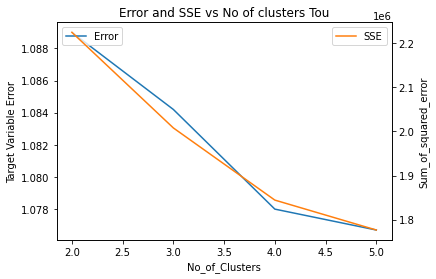
\includegraphics[width=0.5\columnwidth]{hw#4/8.png}
\end{align}
\end{subfigure}
\begin{subfigure}
\begin{align}
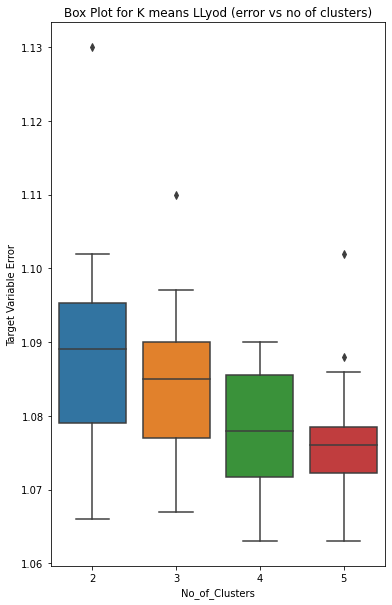
\includegraphics[width=0.5\columnwidth]{hw#4/9.png}
\end{align}
\end{subfigure}
\begin{subfigure}
\begin{align} 
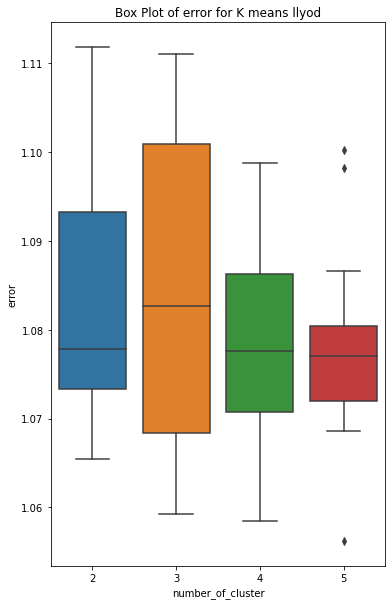
\includegraphics[width=0.5\columnwidth]{hw#4/10.png}
\end{align}
\end{subfigure}
\begin{subfigure}
\begin{align}
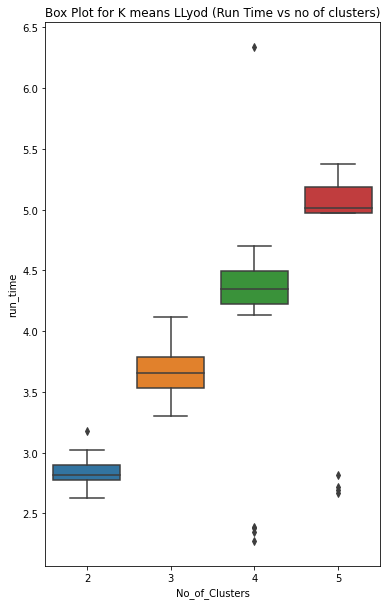
\includegraphics[width=0.5\columnwidth]{hw#4/11.png}       
\end{align}
\end{subfigure}
\textbf{NYC Dataset Graphs}
\begin{subfigure}
\begin{align}
    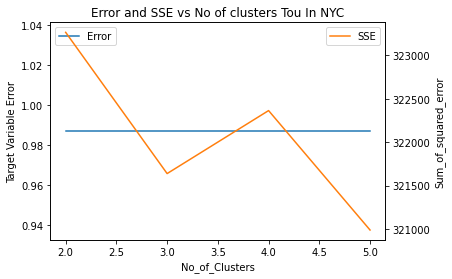
\includegraphics[width=0.5\columnwidth]{hw#4/40.png}
\end{align}    
\end{subfigure}
\begin{subfigure}
\begin{align}
    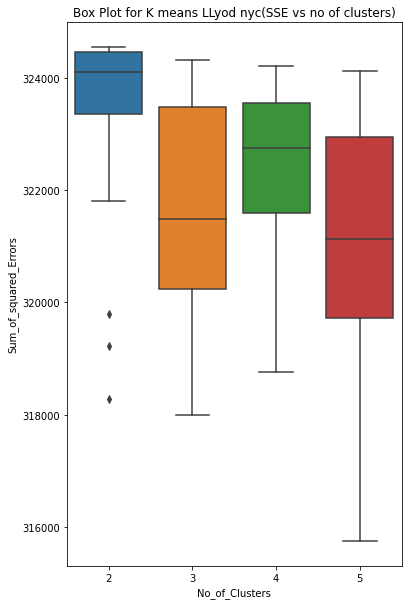
\includegraphics[width=0.5\columnwidth]{hw#4/37.png}
\end{align}    
\end{subfigure}
\begin{subfigure}
\begin{align}
    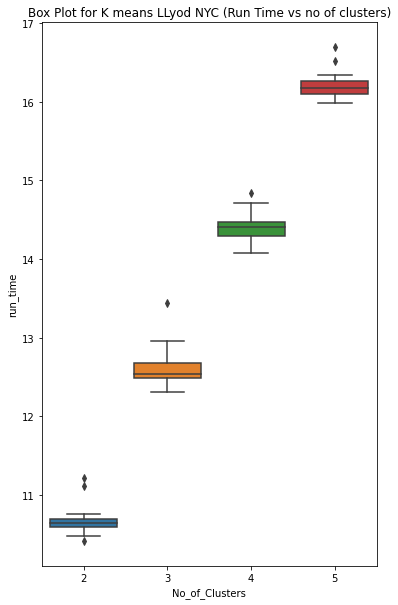
\includegraphics[width=0.5\columnwidth]{hw#4/38.png}
\end{align}    
\end{subfigure}
\subsection{Discussion of Findings}
Answer here$\ldots$
\begin{itemize}
\item \textbf{Method used for representing Comment Body}
\item Since Comment Body column is a free text column, I have 
used Natural Language Processing method to convert the text 
into appropriate vector representation.
\item Applying appropriate pre-processing steps to clean the 
data such as removing stopwords,Stemming-Converting word to 
root word,Removing URLS, Removing punctuations,Removing Non 
alphanumeric letters,Removing Digit, Converting text to lower font.
\item Conversion from text to Vector using Count vectorizer method
\item The reason for using Count Vectorizer method is as follows:
\item CountVectorizer focuses on the frequency of words in a 
document, whereas TF-IDF considers the frequency of words 
across all documents in the dataset. This means that 
CountVectorizer is better suited to capturing the specificity 
of a document, which is important in clustering, where we want to group similar documents together.
\item CountVectorizer is simpler and faster than TF-IDF because 
it only counts the number of occurrences of each word in a 
document, while TF-IDF requires more complex calculations to 
take into account the frequency of words across all documents.
\item CountVectorizer produces integer counts for each word, 
which can be more easily interpreted and used in clustering 
algorithms, compared to the decimal values produced by TF-IDF.
\item In summary, CountVectorizer is a better choice than TF-
IDF for clustering when we want to focus on the specific 
characteristics of each document and need a simpler and faster 
approach to processing large amounts of text data.
\item \textbf{Algorithm Description}
\item The algorithm implemented is K means with a Threshold
\item I have implemented the algorithm for Diabetes dataset as well as NYC comments dataset for clusters 2 to 5 and number of iterations between 1 to 20.
\item The threshold value is set to a low value and when the distances between old centroids and the new centroids have changed and the value is below a threshold the Algorithm stops
\item I have recorded the Graph values for 80 iterations
\item The error value is calculated from the Target Variable,The intuition behind target variable is since we are performing a binary classification, Let that be the original classes.
\item When we increase the number of clusters we have to merge the clusters based on the distance from the original clusters from the input dataframe.
\item \textbf{Merging of N clusters into 2}
\item The merging process calculates the distances between the centroids acheived from clustering and the original dataframe clusters,and it mappes the cluster to the nearest input cluster
\item Thus after performing clustering based on target variable we are able to plot the graph for datasets.

\item \textbf{Conclusions from the Graph}
\item For Diabetes Dataset:From the first graph containing SSE and error with Target Variable we conclude that as number of clusters increase the withing Sum of Square errors tend to decrease.
\item However for the error with the target variable we can see randomness when we run different experiments.
\item In a general case the error tends to balance out when we increase the number of clusters and the imbalances in the classes decrease.
\item The box Plots for the Diabetes Dataset also suggest a similar story, For the Sum of Squared Errors the median value of errors tend to decrease as we increase the clusters.
\item The Box plots of Runtime suggests an increase in runtime as we increase the number of clusters,The median value for a cluster number higher is high.

\item \textbf{Conclusion for NYC Comments Dataset}
\item From the first graph we can conclude that the Sum of Squared Error decreases as we increase the number of clusters
\item After applying pre processing and taking the most frequent 2.9 percent of dataset we can see,After applying count vectorizer Df we generate a sparse matrix of 50 lakh rows and some hundreds columns.
\item Since the matrix is sparse when we try to merge the cluster based on distance metric we get the same distance and hence the Error of target variable remains the same.
\item Because of Sparsity we can see the clusters formed would be homogeneous and hence error with target variable wont change.
\item For the box plots we can see as the number of clusters increase the SSE median becomes low.
\item The Run time generally increases with increase in the cluster.

\item Imrpovements in K means Llyod
\item We can initialize K means in a better way and implement K means ++ centroids initialization thus reducing the Within Cluster Sum of Square Errors
\item We can implement \textbf{Triangle Inequality} to improve the K means Algorithm and remove the needless cluster calculations.



\end{itemize}


\end{homeworkProblem}




%----------------------------------------------------------------------------------------
%	PROBLEM 5
%----------------------------------------------------------------------------------------
\begin{homeworkProblem}

 The $k$-means algorithm provided above stops when centroids become stable (Line  34). In theory, $k$-means converges once SSE is minimized
\begin{eqnarray*}
SSE = \sum_{j}^k \ \ \smashoperator{ \sum_{x \in c_j.B}} ||\mathbf{x} - c_j.v||^2_2 \label{costfunt}
\end{eqnarray*} 


 
In this question, you are asked to use SSE as stopping criterion. Run  your program, $C_{k_{SSE}}$, against the Diabetes and New York Times Comments data sets. Report the total error rates for $k = 2,\ldots 5$ for 20 runs each for both data sets. Moreover, compare k-means and kmeans++'s run time for $k = 2,\ldots 5$ for 20 runs using both data sets. Presenting the results that are easily understandable.  Plots are generally a good way to convey complex ideas quickly, i.e., box plot.  Discuss  your results [\textbf{20 points}].\\ 


\subsection{R/Python script }
\begin{lstlisting}[language=R]
# Sample R Script With Highlighting

\end{lstlisting}

\begin{lstlisting}[language=Python]

import numpy as np
import swifter
from scipy.spatial.distance import euclidean
from scipy.spatial.distance import cdist
import time

         
def get_random_centroids(input_dataframe,no_of_clusters):
    '''
    The function takes a dataframe as an input and creates a 
    random K centroids from uniform distribution
    '''
    #Initialize random centroids from dataset
    list_of_centroids = []
    
    for cluster in range(no_of_clusters):
        #Generates a centroids randomly from uniform distribution 
        random_centroid = input_dataframe.swifter.apply(lambda 
        x:float(x.sample()))
        #From the given dataset it randomly selects centroids
        
        list_of_centroids.append(random_centroid)
    
    centroid_df=pd.concat(list_of_centroids,axis=1)
    #Naming the column as Label for ease of purpose
    centroid_df.index.name='Cluster_Assigned'
    '''
    The function returns a dataframe consisting of no of 
    clusters required
    '''
    return centroid_df

def get_labels(input_dataframe,centroid_df):
    '''
    This function takes centroids as input and takes the 
    initial dataframe and gives them labels to which cluster
    they belong to
    '''
    euclidean_distances = centroid_df.swifter.apply(lambda x: 
    np.sqrt(((input_dataframe - x) ** 2).sum(axis=1)))
    #Here we use idxmin functionality to handle ties in the 
    dataset 
    #and it randomly assigns if euclideab distance results in a 
    tie
    '''
    This function returns the index of minimum distances as a 
    dataframe
    '''
    return pd.DataFrame(euclidean_distances.idxmin(axis=1))

        
def get_new_centroids(df_clustered_label,input_dataframe):
    '''
    The input dataframe is the dataframe with clusters labelled 
    and the original dataframe
    '''
    df_original_label_join=input_dataframe.join(df_clustered_lab
    el)
    #This is a dataframe that consists of datapoints as well as 
    the cluster assigned 
    df_original_label_join.rename(columns={0:'Cluster_Assigned'},inplace=True)
    #To get the new centroids we group by the Label column and 
    take its mean
    
    
    
    new_centroids=df_original_label_join.groupby('Cluster_Assign
    ed').mean()
    #Here transpose is taken to maintain consistency between 
    original random centroids and 
    return new_centroids.T


def 
kmeans_SSE_Convergence(input_dataframe,no_of_clusters,sum_of_squ
ared_threshold,no_of_iterations):
    '''
    Treats K means as an optimization Problem and stops when 
    difference in SSE reaches a threshold
    The input to the function is the dataframe,no of clusters 
    and a threshold which indicates the perecentage change
    It indicates user can set the percentage change in the SSE 
    and once the percentage change in SSE drops to the 
    Threshold we can see the algorithm has converged
    '''
    start_time=time.time()
    iteration=0
    #Step 1 of k means is to get random _Centroids
    initial_centroid=get_random_centroids(input_dataframe,no_of_clusters)
    #Randomly generated centroids would be stored on centroids 
    #Storing the column list to handle K ties 
    initial_centroid_column_list=initial_centroid.columns.to_list()
    #Get initial labels
    df_cluster_label=get_labels(input_dataframe,initial_centroid)
    #Compute the initial Sum of squared Errors
    initial_sum_of_squared_errors=sum_of_square_error_function(d
    f_cluster_label,input_dataframe,initial_centroid,no_of_clust
    ers)
    
    
    while True:
        '''
        The while loop runs until convergence condition is met
        '''
        
        
        df_new_centroids=get_new_centroids(df_cluster_label,inpu
        t_dataframe)
        '''
        Handling (Maintaining K Centroids)
        '''
        new_list_of_columns=df_new_centroids.columns.to_list()
        #Keeping the number of clusters same
        initial_set_columns = set(initial_centroid_column_list)
        new_set_columns = set(new_list_of_columns)
        missing_columns = initial_set_columns - new_set_columns
        for col in missing_columns:
            df_new_centroids[col]=initial_centroid[col]
            
        '''
        Assigning labels to new centroids
        '''
        df_cluster_label_iter=get_labels(input_dataframe,df_new_
        centroids)
        '''
        
        Calculating the current SSE
        
        '''
        
        updated_sum_of_squared_errors=sum_of_square_error_functi
        on(df_cluster_label_iter,input_dataframe,df_new_centroid
        s,no_of_clusters)
        
        
        #Calculating the convergence criteria
        
        percentage_change=((initial_sum_of_squared_errors-
        updated_sum_of_squared_errors)/(initial_sum_of_squared_e
        rrors))*100
        
        iteration+=1
        #Stopping criteria
        #Indicating new clusters have reduced the SSE
        if percentage_change>0:
            if percentage_change>=sum_of_squared_threshold or 
            iteration>no_of_iterations:
                print("The input SSE Threshold was 
                {}".format(sum_of_squared_threshold))
                print("The percentage change is 
                {}".format(percentage_change))
                print("The initial error was {} and final error 
                was 
                {}".format(initial_sum_of_squared_errors,updated
                _sum_of_squared_errors))
                
                error=cluster_error_target_variable(df_cluster_l
                abel_iter,input_dataframe,no_of_clusters,df_new_
                centroids)
                end_time=time.time()
                return 
                df_new_centroids,error,updated_sum_of_squared_er
                rors,end_time-start_time
                break
                
        else:
            initial_centroid= df_new_centroids
            df_cluster_label=df_cluster_label_iter
            initial_sum_of_squared_errors=updated_sum_of_squared
            _errors
        

def 
sum_of_square_error_function(df_cluster_label,input_dataframe,df
_new_centroids,no_of_clusters):
    '''
    This function calculates the euclidean distance between new 
    formed 
    centroids and the datapoints in that cluster
    '''
    df_data_label=input_dataframe.join(df_cluster_label)
    #Renaming the column
    df_data_label.rename(columns={0:'Cluster_Assigned'},inplace=True)
    total_error=[]
    for cluster in range(no_of_clusters):
        
        df_data_label_cluster=df_data_label[df_data_label['Clust
        er_Assigned']==cluster]
        df_data_label_cluster=df_data_label_cluster.drop('Cluste
        r_Assigned',axis=1)
        centroids=pd.DataFrame(df_new_centroids[cluster])
        euclidean_distance=cdist(df_data_label_cluster,centroids
        .T,metric='euclidean')
        
        total_error.append(sum(euclidean_distance))
    return round(float(''.join(map(str, sum(total_error)))),3)
        
        
        
def 
cluster_error_target_variable(df_cluster_label,input_dataframe,n
o_of_clusters,df_new_centroids):
    '''
    This calculates the error for every cluster and sums up the 
    error based on the formula for error
    '''
    
    target_variable_centroid=input_dataframe.groupby('readmitted').mean().reset_index()
    '''
    Target variable centroid is input dataframe taking mean
    '''
    new_centroids= df_new_centroids.T
    #
    df_data_label=input_dataframe.join(df_cluster_label)
    #Renaming the column
    df_data_label.rename(columns={0:'Cluster_Assigned'},inplace=True)

    # Get the columns of the data dataframe
    columns = input_dataframe.columns

    sum_of_square_Error= []
    # Compute the distance between each data point and its 
    assigned centroid
    for i in range(len(new_centroids)):   
        s=[]
        for j in range(len(target_variable_centroid)): ### mean centroid
            #Calculating the error between target variable 
            centroid and new centroids
            distance = 
            np.sum(np.square(target_variable_centroid[target_var
            iable_centroid['readmitted']==j][columns] - 
            new_centroids.iloc[i][columns]), axis=1)
            
            #Storing the distance
            s.append(distance.iloc[0])
        sum_of_square_Error.append(s)
    
    
    merged_new_label=pd.DataFrame(sum_of_square_Error).idxmin(ax
    is=1)
    
    #Merging of cluster
    mapping_dictionary=merged_new_label.to_dict() 
    
    #Getting clusters to a new column
    df_data_label['target_variable_cluster']=df_data_label['Clus
    ter_Assigned'].replace(mapping_dictionary)
    
    
    total_cluster_error = []
    
    for class_name in range(0,2):
        df_cluster = 
        df_data_label[df_data_label['target_variable_cluster'] == class_name] 
        yi = len(df_cluster[df_cluster['readmitted'] == 1]) 
        #Calculating Ni
        ni = len(df_cluster[df_cluster['readmitted'] == 0]) 
        if yi == 0 and ni == 0:
            error_ci = 0
        else:
            error_ci = ni / (ni + yi) # calculate the error rate of the current cluster
        total_cluster_error.append(error_ci)
    return round(sum(total_cluster_error),3)
error_values_kmeans_convergence=[]
for no_of_clusters in range(2,6):
    #Taking the cluster value from 2 to 5
    for no_of_experiments in range(1,21):
        #Performing experiments for each cluster 20 times
        final_centroids,error_target_variable,sum_of_squared_err
        or,run_time=kmeans_SSE_Convergence(df_diabetes_final,no_
        of_clusters,10,100)
        #Storing the variables in dataframe
        error_values_kmeans_convergence.append([no_of_clusters,n
        o_of_experiments,error_target_variable,sum_of_squared_er
        ror,run_time])
error_values_kmeans_convergence_df= 
pd.DataFrame(error_values_kmeans_convergence,columns=
['No_of_Clusters', 'Iteration Number', 'Target Variable 
Error','Sum_of_squared_Errors','run_time'])  

 No_of_Clusters 	Iteration Number 	Target Variable Error 	
 Sum_of_squared_Errors 	run_time
0 	2 	1 	1.066 	2413170.508 	2.726349
1 	2 	2 	1.078 	2287579.727 	2.718648
2 	2 	3 	1.087 	2182532.040 	2.797202
3 	2 	4 	1.104 	2221605.043 	2.712034
4 	2 	5 	1.091 	2189499.368 	2.718228
5 	2 	6 	1.079 	2277045.553 	2.694952
6 	2 	7 	1.061 	2303720.984 	2.644690
7 	2 	8 	1.088 	2170057.769 	2.651664
8 	2 	9 	1.095 	2200394.800 	2.699285
9 	2 	10 	1.072 	2267420.702 	2.626602
10 	2 	11 	1.090 	2193666.813 	2.684914
11 	2 	12 	1.077 	2246487.630 	2.642030
12 	2 	13 	1.082 	2171039.014 	2.644447
13 	2 	14 	1.081 	2174714.967 	2.745272
14 	2 	15 	1.083 	2170344.044 	2.783290
15 	2 	16 	1.075 	2189936.038 	2.729855
16 	2 	17 	1.101 	2340073.186 	2.873033
17 	2 	18 	1.076 	2233414.214 	2.730305
18 	2 	19 	1.102 	2214350.488 	2.810346
19 	2 	20 	1.073 	2186929.281 	2.714788
20 	3 	1 	1.065 	1935225.192 	3.246217
21 	3 	2 	1.101 	2039320.017 	3.350098
22 	3 	3 	1.083 	1968438.520 	3.402092
23 	3 	4 	1.079 	1995877.788 	3.405518
24 	3 	5 	1.068 	1961866.877 	3.464136
25 	3 	6 	1.086 	2064005.550 	3.408696
26 	3 	7 	1.080 	1925746.674 	3.363921
27 	3 	8 	1.064 	1958785.399 	3.420779
28 	3 	9 	1.086 	1954132.773 	3.441963
29 	3 	10 	1.063 	1959673.274 	3.389995
30 	3 	11 	1.105 	1967024.521 	3.409568
31 	3 	12 	1.094 	2063132.009 	3.410118
32 	3 	13 	1.059 	1977468.991 	3.503200
33 	3 	14 	1.060 	2009608.064 	3.329814
34 	3 	15 	1.091 	2067597.639 	3.413102
35 	3 	16 	1.064 	2139787.389 	3.337727
36 	3 	17 	1.114 	1997694.204 	3.381265
37 	3 	18 	1.077 	2030874.333 	3.305255
38 	3 	19 	1.069 	1944534.045 	3.378402
39 	3 	20 	1.069 	2134921.766 	3.388444
40 	4 	1 	1.069 	1903662.597 	4.067786
41 	4 	2 	1.103 	1857357.414 	3.997676
42 	4 	3 	1.087 	1878725.172 	4.159650
43 	4 	4 	1.105 	1880647.531 	4.119273
44 	4 	5 	1.061 	1861897.586 	4.022799
45 	4 	6 	1.061 	1807974.571 	4.102464
46 	4 	7 	1.085 	1984950.693 	4.216363
47 	4 	8 	1.078 	1824653.970 	4.038547
48 	4 	9 	1.073 	1924015.710 	4.060449
49 	4 	10 	1.070 	1832468.147 	4.123883
50 	4 	11 	1.088 	2021315.876 	4.306999
51 	4 	12 	1.087 	1892568.867 	4.296274
52 	4 	13 	1.066 	1864108.356 	4.136086
53 	4 	14 	1.070 	1812281.605 	4.087149
54 	4 	15 	1.071 	1800758.124 	4.172847
55 	4 	16 	1.073 	1824418.302 	4.047086
56 	4 	17 	1.058 	1897934.940 	4.181204
57 	4 	18 	1.079 	1817142.740 	4.077854
58 	4 	19 	1.089 	1934103.757 	4.013173
59 	4 	20 	1.103 	1939041.632 	4.106091
60 	5 	1 	1.082 	1743442.199 	4.785248
61 	5 	2 	1.068 	1660872.055 	4.651742
62 	5 	3 	1.091 	1808287.699 	4.656569
63 	5 	4 	1.084 	1773047.315 	4.665026
64 	5 	5 	1.066 	1844519.156 	4.706286
65 	5 	6 	1.076 	1740907.723 	4.691701
66 	5 	7 	1.081 	1777958.584 	4.754583
67 	5 	8 	1.072 	1781775.749 	4.818693
68 	5 	9 	1.089 	1775093.996 	4.787339
69 	5 	10 	1.089 	1680293.631 	4.772455
70 	5 	11 	1.068 	1689785.267 	4.638578
71 	5 	12 	1.086 	1799536.909 	4.668274
72 	5 	13 	1.074 	1768360.548 	4.687613
73 	5 	14 	1.075 	1777205.297 	4.677921
74 	5 	15 	1.075 	1767950.472 	4.691387
75 	5 	16 	1.071 	1744607.719 	4.769310
76 	5 	17 	1.092 	1678438.903 	4.748329
77 	5 	18 	1.080 	1800264.784 	4.680258
78 	5 	19 	1.088 	1892715.711 	4.720975
79 	5 	20 	1.076 	1757773.294 	4.669850


error_values_kmeans_convergence=error_values_kmeans_convergence_
df.groupby(['No_of_Clusters']).mean().reset_index()
[['No_of_Clusters','Target Variable 
Error','Sum_of_squared_Errors','run_time']]
error_values_kmeans_convergence    

No_of_Clusters 	Target Variable Error 	Sum_of_squared_Errors 	
run_time
0 	2 	1.08305 	2.231699e+06 	2.717397
1 	3 	1.07885 	2.004786e+06 	3.387516
2 	4 	1.07880 	1.878001e+06 	4.116683
3 	5 	1.07915 	1.763142e+06 	4.712107

#NYC DATASET


import numpy as np
import swifter
from scipy.spatial.distance import euclidean
from scipy.spatial.distance import cdist
import time

         
def get_random_centroids(input_dataframe,no_of_clusters):
    '''
    The function takes a dataframe as an input and creates a 
    random K centroids from uniform distribution
    '''
    #Initialize random centroids from dataset
    list_of_centroids = []
    
    for cluster in range(no_of_clusters):
        #Generates a centroids randomly from uniform 
        distribution 
        random_centroid = input_dataframe.swifter.apply(lambda x:float(x.sample()))
        #From the given dataset it randomly selects centroids
        list_of_centroids.append(random_centroid)
    
    centroid_df=pd.concat(list_of_centroids,axis=1)
    #Naming the column as Label for ease of purpose
    centroid_df.index.name='Cluster_Assigned'
    '''
    The function returns a dataframe consisting of no of 
    clusters required
    '''
    return centroid_df

def get_labels(input_dataframe,centroid_df):
    '''
    This function takes centroids as input and takes the 
    initial dataframe and gives them labels to which cluster
    they belong to
    '''
    euclidean_distances = centroid_df.swifter.apply(lambda x: 
    np.sqrt(((input_dataframe - x) ** 2).sum(axis=1)))
    #Here we use idxmin functionality to handle ties in the 
    dataset 
    #and it randomly assigns if euclideab distance results in a 
    tie
    '''
    This function returns the index of minimum distances as a dataframe
    '''
    return pd.DataFrame(euclidean_distances.idxmin(axis=1))

        
def get_new_centroids(df_clustered_label,input_dataframe):
    '''
    The input dataframe is the dataframe with clusters labelled 
    and the original dataframe
    '''
    
    df_original_label_join=input_dataframe.join(df_clustered_lab
    el)
    #This is a dataframe that consists of datapoints as well as the cluster assigned 
    df_original_label_join.rename(columns=
    {0:'Cluster_Assigned'},inplace=True)
    #To get the new centroids we group by the Label column and take its mean
    new_centroids=df_original_label_join.groupby('Cluster_Assign
    ed').mean()
    #Here transpose is taken to maintain consistency between 
    original random centroids and 
    return new_centroids.T


def 
kmeans_SSE_Convergence(input_dataframe,no_of_clusters,sum_of_squ
ared_threshold,no_of_iterations):
    '''
    Treats K means as an optimization Problem and stops when 
    difference in SSE reaches a threshold
    The input to the function is the dataframe,no of clusters 
    and a threshold which indicates the perecentage change
    It indicates user can set the percentage change in the SSE 
    and once the percentage change in SSE drops to the 
    Threshold we can see the algorithm has converged
    '''
    start_time=time.time()
    iteration=0
    #Step 1 of k means is to get random _Centroids
    initial_centroid=get_random_centroids(input_dataframe,no_of_
    clusters)
    #Randomly generated centroids would be stored on centroids 
    #Storing the column list to handle K ties 
    initial_centroid_column_list=initial_centroid.columns.to_lis
    t()
    #Get initial labels
    df_cluster_label=get_labels(input_dataframe,initial_centroid
    )
    #Compute the initial Sum of squared Errors
    initial_sum_of_squared_errors=sum_of_square_error_function(d
    f_cluster_label,input_dataframe,initial_centroid,no_of_clust
    ers)
    
    
    while True:
        '''
        The while loop runs until convergence condition is met
        '''
        
        df_new_centroids=get_new_centroids(df_cluster_label,inpu
        t_dataframe)
        '''
        Handling (Maintaining K Centroids)
        '''
        new_list_of_columns=df_new_centroids.columns.to_list()
        #Keeping the number of clusters same
        initial_set_columns = set(initial_centroid_column_list)
        new_set_columns = set(new_list_of_columns)
        missing_columns = initial_set_columns - new_set_columns
        for col in missing_columns:
            df_new_centroids[col]=initial_centroid[col]
            
        '''
        Assigning labels to new centroids
        '''
        df_cluster_label_iter=get_labels(input_dataframe,df_new_
        centroids)
        '''
        Calculating the current SSE
        
        '''
        updated_sum_of_squared_errors=sum_of_square_error_functi
        on(df_cluster_label_iter,input_dataframe,df_new_centroid
        s,no_of_clusters)
        
        #Calculating the convergence criteria
        
        percentage_change=((initial_sum_of_squared_errors-
        updated_sum_of_squared_errors)/(initial_sum_of_squared_e
        rrors))*100
        
        iteration+=1
        #Stopping criteria
        #Indicating new clusters have reduced the SSE
        if percentage_change>0:
            if percentage_change>=sum_of_squared_threshold or 
            iteration>no_of_iterations:
                print("The input SSE Threshold was 
                {}".format(sum_of_squared_threshold))
                print("The percentage change is 
                {}".format(percentage_change))
                print("The initial error was {} and final error 
                was 
                {}".format(initial_sum_of_squared_errors,updated
                _sum_of_squared_errors))
                
                error=cluster_error_target_variable(df_cluster_l
                abel_iter,input_dataframe,no_of_clusters,df_new_
                centroids)
                end_time=time.time()
                return df_new_centroids,error,updated_sum_of_squared_er
                rors,end_time-start_time
                break
                
        else:
            initial_centroid= df_new_centroids
            df_cluster_label=df_cluster_label_iter
            initial_sum_of_squared_errors=updated_sum_of_squared_errors
        

def sum_of_square_error_function(df_cluster_label,input_dataframe,df
_new_centroids,no_of_clusters):
    '''
    This function calculates the euclidean distance between new formed 
    centroids and the datapoints in that cluster
    '''
    df_data_label=input_dataframe.join(df_cluster_label)
    #Renaming the column
    df_data_label.rename(columns=
    {0:'Cluster_Assigned'},inplace=True)
    total_error=[]
    for cluster in range(no_of_clusters):
        df_data_label_cluster=df_data_label[df_data_label['Cluster_Assigned']==cluster]
        df_data_label_cluster=df_data_label_cluster.drop('Cluster_Assigned',axis=1)
        centroids=pd.DataFrame(df_new_centroids[cluster])
        euclidean_distance=cdist(df_data_label_cluster,centroids.T,metric='euclidean')
        total_error.append(np.nansum(euclidean_distance))
    
    return round(np.nansum(total_error),3)
        
        
        
def 
cluster_error_target_variable(df_cluster_label,input_dataframe,n
o_of_clusters,df_new_centroids):
    '''
    This calculates the error for every cluster and sums up the 
    error based on the formula for error
    '''
    
    target_variable_centroid=input_dataframe.groupby('editorsSelection').mean().reset_index()
    '''
    Target variable centroid is input dataframe taking mean
    '''
    new_centroids= df_new_centroids.T
    #
    df_data_label=input_dataframe.join(df_cluster_label)
    #Renaming the column
    df_data_label.rename(columns={0:'Cluster_Assigned'},inplace=True)

    # Get the columns of the data dataframe
    columns = input_dataframe.columns

    sum_of_square_Error= []
    # Compute the distance between each data point and its assigned centroid
    for i in range(len(new_centroids)):   
        s=[]
        for j in range(len(target_variable_centroid)): ### mean centroid
            #Calculating the error between target variable 
            centroid and new centroids
            distance = 
            np.sum(np.square(target_variable_centroid[target_var
            iable_centroid['editorsSelection']==j][columns] - 
            new_centroids.iloc[i][columns]), axis=1)
            #Storing the distance
            s.append(distance.iloc[0])
        sum_of_square_Error.append(s)
    
    
    merged_new_label=pd.DataFrame(sum_of_square_Error).idxmin(axis=1)
    
    #Merging of cluster
    mapping_dictionary=merged_new_label.to_dict() 
    
    #Getting clusters to a new column
   
    df_data_label['target_variable_cluster']=
    df_data_label['Clus
    ter_Assigned'].replace(mapping_dictionary)
    
    
    total_cluster_error = []
    
    for class_name in range(0,2):
        df_cluster = df_data_label[df_data_label['target_variable_cluster'] == class_name] 
        yi = len(df_cluster[df_cluster['editorsSelection'] == 1]) 
        #Calculating Ni
        ni = len(df_cluster[df_cluster['editorsSelection'] == 0]) 
        if yi == 0 and ni == 0:
            error_ci = 0
        else:
            error_ci = ni / (ni + yi) # calculate the error rate of the current cluster
        total_cluster_error.append(error_ci)
    return round(sum(total_cluster_error),3)
error_values_kmeans_convergence=[]
for no_of_clusters in range(2,6):
    #Taking the cluster value from 2 to 5
    for no_of_experiments in range(1,21):
        #Performing experiments for each cluster 20 times
        
        final_centroids,error_target_variable,sum_of_squared_err
        or,run_time=kmeans_SSE_Convergence(count_vectorizer_df,n
        o_of_clusters,10,100)
        #Storing the variables in dataframe
        error_values_kmeans_convergence.append([no_of_clusters,n
        o_of_experiments,error_target_variable,sum_of_squared_er
        ror,run_time])
error_values_kmeans_convergence_df_full= 
pd.DataFrame(error_values_kmeans_convergence,columns=
['No_of_Clusters', 'Iteration Number', 'Target Variable 
Error','Sum_of_squared_Errors','run_time'])  
error_values_kmeans_convergence_df_full.to_csv('nyc_Sse_data.csv
')    
No_of_Clusters 	Iteration Number 	Target Variable Error 	
Sum_of_squared_Errors 	run_time
0 	2 	1 	0.987 	317878.061 	19.744410
1 	2 	2 	0.987 	323528.786 	19.373257
2 	2 	3 	0.987 	324554.100 	19.070758
3 	2 	4 	0.987 	324551.914 	20.030429
4 	2 	5 	0.987 	323339.223 	18.989385
... 	... 	... 	... 	... 	...
75 	5 	16 	0.987 	315650.628 	38.673154
76 	5 	17 	0.987 	314343.849 	39.018158
77 	5 	18 	0.987 	312601.780 	38.846771
78 	5 	19 	0.987 	314152.048 	37.687718
79 	5 	20 	0.987 	317688.822 	39.600342

80 rows × 5 columns
\end{lstlisting}



\subsection{Plots }
\textbf{Diabetes Dataset}
\begin{subfigure}

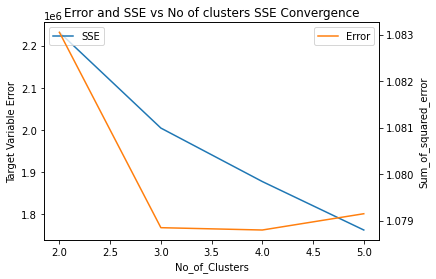
\includegraphics[width=0.5\columnwidth]{hw#4/12.png}
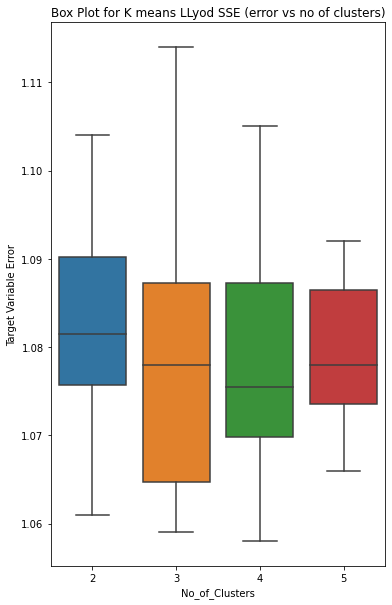
\includegraphics[width=0.5\columnwidth]{hw#4/13.png}
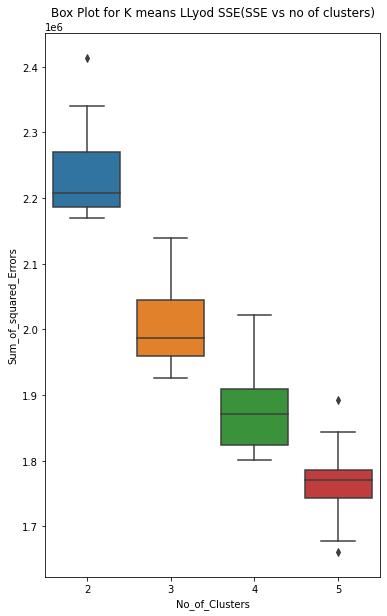
\includegraphics[width=0.5\columnwidth]{hw#4/14.png}
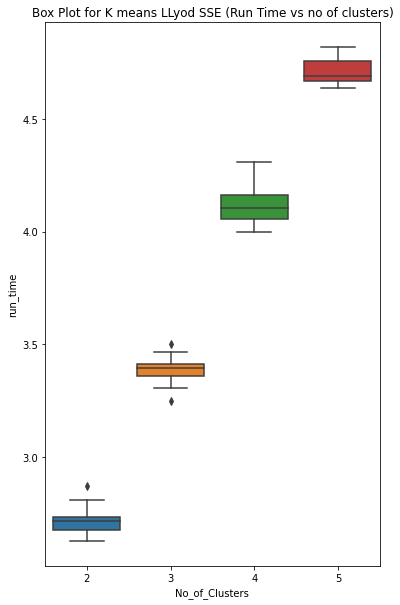
\includegraphics[width=0.5\columnwidth]{hw#4/15.png}

\end{subfigure}
\textbf{NYC DATASET}
\begin{subfigure}
\begin{align}
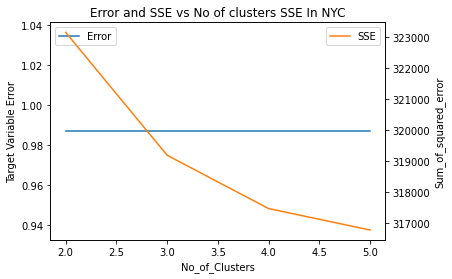
\includegraphics[width=0.5\columnwidth]{hw#4/41.png}    
\end{align}
\begin{subfigure}
\begin{align}
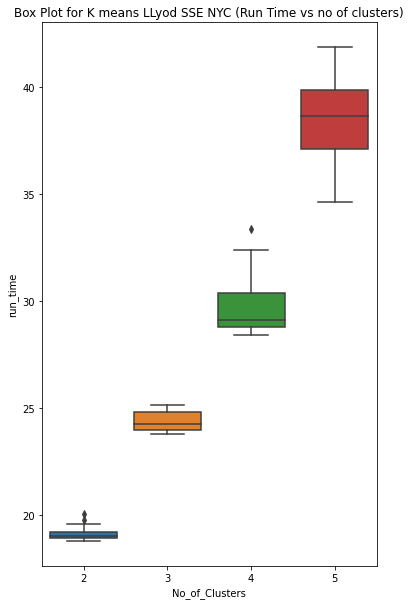
\includegraphics[width=0.5\columnwidth]{hw#4/33.png} 
\end{align}
\end{subfigure}
\begin{subfigure}
\begin{align}
    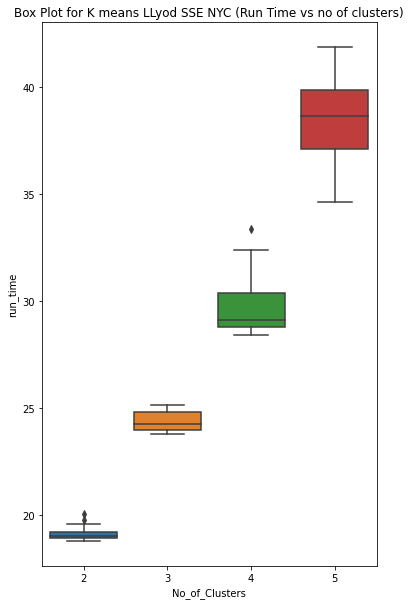
\includegraphics[width=0.5\columnwidth]{hw#4/33.png}
\end{align}    
\end{subfigure}
\begin{subfigure}
    \begin{align}
        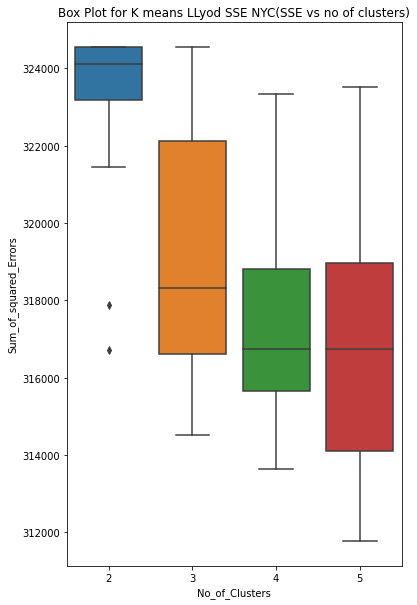
\includegraphics[width=0.5\columnwidth]{hw#4/34.png}
    \end{align}
\end{subfigure}
\begin{subfigure}
\begin{align}
    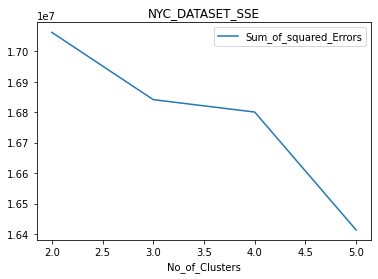
\includegraphics[width=0.5\columnwidth]{hw#4/35.png}
    \end{align}
\end{subfigure}

\end

\subsection{Discussion of Findings}
\begin{itemize}
    \item Changed the convergence criteria using SSE
    \item \textbf{The covergence criteria decided is} At every single iteration we calculate the Within Sum of Square Errors and when the Sum of Square errors between cluster assigned drops to 10 percent from the previous cluster our algorithm converges
    \item It is a customizable code with the threshold can be decided by the user and when the difference between SSE drops to a certain user specified value the convergence takes place and the algorithm stops.
    \item However the algorithm is susceptible to random cluster initialization and it depends on the first cluster selected.
    \item After running the algorithm on Diabetes dataset as well as New york Comments Dataset we can conclude
    \item For the Diabetes dataset the SSE decrease as we increase the cluster.
    \item The target value error decreases when the number of clusters are three and it balances later
    \item However due to randomness the target value error shows different graphs based on merging strategy and the general trend is it stabilizes and the classes tend to balance
    \item From the graph of runtime and box plots we can conclude as the number of clusters increase the run time also increase

    \item For the NYC dataset we can conclude due to sparsity in the dataset it leads to homogeneous clusters and thus the target value error remains constant.
    \item The run time increases as the number of clusters increases and thus the median value of run time increases with increase in cluster

    \item \textbf{Comparisons for the graphs} 
    \item SSE convergence is generally considered the better 
    metric to use because it directly measures the quality of 
    the clustering. Convergence of the change of centroids can 
    be influenced by factors such as the initial positions of 
    the centroids and the number of clusters.
    \item 


    \item In summary, SSE convergence is a better metric to use 
    in K-means than convergence of the change of centroids as 
    it provides a more direct measurement of the quality of 
    clustering.

\end{itemize}

\end{homeworkProblem}
%----------------------------------------------------------------------------------------
%	PROBLEM 6
%----------------------------------------------------------------------------------------

\begin{homeworkProblem}
Traditional $k$-means initialization is based on choosing values from a uniform distribution. In this question, you are asked to improve $k$-means through initialization.  \href{http://ilpubs.stanford.edu:8090/778/1/2006-13.pdf}{$k$-means ++} is an extended $k$-means clustering algorithm and induces non-uniform  distributions over  the data  that serve as  the initial centroids. Read the paper and discuss the idea in a paragraph.  Implement this idea to improve your $k$-means program. Run  your program, $C_{k++}$, against the Diabetes and New York Times Comments data sets. Report the total error rates for $k = 2,\ldots 5$ for 20 runs each for both data sets. Moreover, compare $C_{k}$, $C_{k_{SSE}}$ and $C_{k++}$'s run time for $k = 2,\ldots 5$ for 20 runs using both data sets. Presenting the results that are easily understandable.  Plots are generally a good way to convey complex ideas quickly, i.e., box plot.  Discuss  your results [\textbf{20 points}].\\ 


\subsection{R/Python script }
\begin{lstlisting}[language=R]
# Sample R Script With Highlighting

\end{lstlisting}

\begin{lstlisting}[language=Python]

import numpy as np
import swifter
from scipy.spatial.distance import euclidean
from scipy.spatial.distance import cdist
import time

def kmeans_pp_init(input_dataframe,no_of_clusters):
    '''
    K-means++ is a variant of the K-means algorithm that aims 
    to improve the initial centroids' selection 
    in the clustering process. 
    The standard K-means algorithm initializes the cluster 
    centroids randomly, 
    which can lead to suboptimal clustering results, 
    
    especially if the dataset has complex or irregular 
    structures.
    '''
    list_of_centroids=[]
    #Choosing the first centroid randomly
    centroid = input_dataframe.apply(lambda x: float(x.sample()))
    list_of_centroids.append(centroid)
    
    iterator=2
    while iterator<=no_of_clusters:
        '''
        Calculating the distances from the centroid to every 
        data point
        If the no of centroids are more than 1 calculate the 
        distance from every centroid and take minimum distance
        '''
        distances = 
        np.array(np.amin(cdist(input_dataframe,list_of_centroids
        ,metric='euclidean'),axis=1))
        #Next centroid will be selected with probability 
        proportional to the distance
        
        probs = distances / np.sum(distances)
        '''
        Selection of the next centroids
        '''
        next_centroid = input_dataframe.iloc[np.random.choice(len(input_datafram
        e),p=probs)]
        list_of_centroids.append(next_centroid)
        iterator+=1
    
    
    centroid_df=pd.concat(list_of_centroids,axis=1,ignore_index=True)
    #Naming the column as Label for ease of purpose
    centroid_df.index.name='Cluster_Assigned'   
    
        
    return centroid_df

def get_labels(input_dataframe,centroid_df):
    '''
    This function takes centroids as input and takes the 
    initial dataframe and gives them labels to which cluster
    
    they belong to
    '''
    euclidean_distances = centroid_df.swifter.apply(lambda x: 
    np.sqrt(((input_dataframe - x) ** 2).sum(axis=1)))
    #Here we use idxmin functionality to handle ties in the 
    dataset 
    #and it randomly assigns if euclideab distance results in a 
    tie
    '''
    This function returns the index of minimum distances as a 
    dataframe
    '''
    return pd.DataFrame(euclidean_distances.idxmin(axis=1))

        
def get_new_centroids(df_clustered_label,input_dataframe):
    '''
    The input dataframe is the dataframe with clusters labelled 
    and the original dataframe
    '''
    df_original_label_join=input_dataframe.join(df_clustered_lab
    el)
    #This is a dataframe that consists of datapoints as well as 
    the cluster assigned 
    df_original_label_join.rename(columns=
    {0:'Cluster_Assigned'},inplace=True)
    #To get the new centroids we group by the Label column 
    and take its mean
    new_centroids=df_original_label_join.groupby('Cluster_Assign
    ed').mean()
    #Here transpose is taken to maintain consistency between original random centroids and 
    return new_centroids.T


def kmeans_plus_plus(input_dataframe,no_of_clusters,threshold,no_of_iterations):
    '''
    This function takes original dataframe,number of clusters,threshold as input.
    '''
    start_time=time.time()
    iteration=0
    #Step 1 of k means ++ is to get K means plus plus 
    initialization centroids
    
    initial_centroid=kmeans_pp_init(input_dataframe,no_of_cluste
    rs)
    #Randomly generated centroids would be stored on centroids 
    #Storing the column list to handle K ties 
    
    initial_centroid_column_list=initial_centroid.columns.to_lis
    t()
    
    while True:
        '''
        The while loop runs until convergence condition is met
        '''
        
        df_cluster_label=get_labels(input_dataframe,initial_cent
        roid)
        df_new_centroids=get_new_centroids(df_cluster_label,inpu
        t_dataframe)
        '''
        Handling (Maintaining K Centroids)
        '''
        new_list_of_columns=df_new_centroids.columns.to_list()
        #Keeping the number of clusters same
        initial_set_columns = set(initial_centroid_column_list)
        new_set_columns = set(new_list_of_columns)
        missing_columns = initial_set_columns - new_set_columns
        for col in missing_columns:
            df_new_centroids[col]=initial_centroid[col]
        
        from scipy.spatial.distance import euclidean
        scalar_product = 
        [euclidean(initial_centroid[col],df_new_centroids[col]) 
        for col in initial_centroid.columns]
        threshold_calculated=float(sum(scalar_product))/no_of_cl
        usters
        
        
        iteration+=1
        
        if threshold_calculated<threshold:
            print("The input Threshold was 
            {}".format(threshold))
            print("The calculated threshold is 
            {}".format(threshold_calculated))
        
        if iteration>no_of_iterations:
            print("Limit for iterations has exceeded")
        
        if threshold_calculated<threshold or iteration>no_of_iterations:
            
            error=cluster_error_target_variable(df_cluster_label
            ,input_dataframe,no_of_clusters,df_new_centroids)
            sum_of_square_error=sum_of_square_error_function(df_
            cluster_label,input_dataframe,df_new_centroids,no_of
            _clusters)
            end_time=time.time()
            return 
            df_new_centroids,error,sum_of_square_error,end_time-
            start_time
            break
        else:
            initial_centroid= df_new_centroids
        

def 
sum_of_square_error_function(df_cluster_label,input_dataframe,df
_new_centroids,no_of_clusters):
    '''
    This function calculates the euclidean distance between new 
    formed 
    centroids and the datapoints in that cluster
    '''
    
    df_data_label=input_dataframe.join(df_cluster_label)
    #Renaming the column
    df_data_label.rename(columns=
    {0:'Cluster_Assigned'},inplace=True)
    total_error=[]
    for cluster in range(no_of_clusters):
        
        df_data_label_cluster=df_data_label[df_data_label['Clust
        er_Assigned']==cluster]
        df_data_label_cluster=df_data_label_cluster.drop('Cluste
        r_Assigned',axis=1)
        centroids=pd.DataFrame(df_new_centroids[cluster])
        
        euclidean_distance=cdist(df_data_label_cluster,centroids
        .T,metric='euclidean')
        
        total_error.append(sum(euclidean_distance))
    return round(float(''.join(map(str, sum(total_error)))),3)
        
        
        
def 
cluster_error_target_variable(df_cluster_label,input_dataframe,n
o_of_clusters,df_new_centroids):
    '''
    This calculates the error for every cluster and sums up the 
    error based on the formula for error
    '''
    
    target_variable_centroid=input_dataframe.groupby('readmitted
    
  
    ').mean().reset_index()
    '''
    
    Target variable centroid is input dataframe taking mean
    '''
    new_centroids= df_new_centroids.T
    #
    df_data_label=input_dataframe.join(df_cluster_label)
    #Renaming the column
    df_data_label.rename(columns=
    {0:'Cluster_Assigned'},inplace=True)

    # Get the columns of the data dataframe
    columns = input_dataframe.columns

    sum_of_square_Error= []
    # Compute the distance between each data point and its assigned centroid
    for i in range(len(new_centroids)):   
        s=[]
        for j in range(len(target_variable_centroid)): ### mean 
        centroid
            #Calculating the error between target variable centroid and new centroids
            distance = 
            np.sum(np.square(target_variable_centroid[target_var
            iable_centroid['readmitted']==j][columns] - 
            new_centroids.iloc[i][columns]), axis=1)
            
            #Storing the distance
            s.append(distance.iloc[0])
        sum_of_square_Error.append(s)
    
    
    
    merged_new_label=pd.DataFrame(sum_of_square_Error).idxmin(ax
    is=1)
    
    #Merging of cluster
    
    mapping_dictionary=merged_new_label.to_dict() 
    
    #Getting clusters to a new column
    df_data_label['target_variable_cluster']=df_data_label['Clus
    ter_Assigned'].replace(mapping_dictionary)
    
    
    total_cluster_error = []
    
    for class_name in range(0,2):
        df_cluster = 
        df_data_label[df_data_label['target_variable_cluster'] 
        == class_name] 
        yi = len(df_cluster[df_cluster['readmitted'] == 1]) 
        #Calculating Ni
        ni = len(df_cluster[df_cluster['readmitted'] == 0]) 
        if yi == 0 and ni == 0:
            error_ci = 0
        else:
            error_ci = ni / (ni + yi) # calculate the error 
            rate of the current cluster
        
        total_cluster_error.append(error_ci)
    return round(sum(total_cluster_error),3)
error_values_kmeans_plus_plus=[]
for no_of_clusters in range(2,6):
    #Taking the cluster value from 2 to 5
    for no_of_experiments in range(1,21):
        #Performing experiments for each cluster 20 times
        final_centroids,error_target_variable,sum_of_squared_err
        or,run_time=kmeans_plus_plus(df_diabetes_final,no_of_clu
        sters,10,100)
        #Storing the variables in dataframe
        error_values_kmeans_plus_plus.append([no_of_clusters,no_
        
        
        of_experiments,error_target_variable,sum_of_squared_erro
        r,run_time])
error_values_kmeans_plus_plus_df= 
pd.DataFrame(error_values_kmeans_plus_plus,columns=
['No_of_Clusters', 'Iteration Number', 'Target Variable 
Error','Sum_of_squared_Errors','run_time'])  
error_plot_kmeans_plus_plus=error_values_kmeans_plus_plus_df.gro
upby(['No_of_Clusters']).mean().reset_index()
[['No_of_Clusters','Target Variable 
Error','Sum_of_squared_Errors','run_time']]
error_plot_kmeans_plus_plus
import seaborn as sns
plt.figure(figsize=(6, 10))
#Plotting Box plot
#Plotting values of errors for 80 iterations
sns.boxplot(x=error_values_kmeans_plus_plus_df['No_of_Clusters']
,y=error_values_kmeans_plus_plus_df['Target Variable Error'])
plt.title('Box Plot for K means LLyod K++ (error vs no of 
clusters)')
plt.show()
import seaborn as sns
plt.figure(figsize=(6, 10))
#Plotting Box plot
#Plotting values of errors for 80 iterations
sns.boxplot(x=error_values_kmeans_plus_plus_df['No_of_Clusters']
,y=error_values_kmeans_plus_plus_df['Sum_of_squared_Errors'])
plt.title('Box Plot for K means LLyod k++(SSE vs no of 
clusters)')
plt.show()
import seaborn as sns
plt.figure(figsize=(6, 10))
#Plotting Box plot
#Plotting values of errors for 80 iterations
sns.boxplot(x=error_values_kmeans_plus_plus_df['No_of_Clusters']
,y=error_values_kmeans_plus_plus_df['run_time'])
plt.title('Box Plot for K means LLyod k++(Run Time vs no of 
clusters)')
plt.show()


#Run time comparison
error_values_kmeans_convergence['Algorithm_Used']='K_Means_SSE_o
nvergence'
error_plot_kmeans_plus_plus['Algorithm_Used']='K++Initializatio'
error_plot['Algorithm_Used']='Llyod_Kmeans'

k_means_metric=pd.concat([error_values_kmeans_convergence,error_
plot_kmeans_plus_plus,error_plot],axis=0)
k_means_metric

sns.lineplot(x="No_of_Clusters", 
y="Sum_of_squared_Errors",hue="Algorithm_Used", 
data=k_means_metric)
plt.title('Diabetes_dataset_Comparison)
plt.show()

sns.lineplot(x="No_of_Clusters", y="Sum_of_squared_Errors", 
hue="Algorithm_Used", data=k_means_metric)
plt.title('Diabetes_Dataset_Comparison')
plt.show()
sns.barplot(x="No_of_Clusters", y="Sum_of_squared_Errors", 
hue="Algorithm_Used", data=k_means_metric)
plt.title('Diabetes_Dataset_SSE_Comparison')
plt.show()
sns.barplot(x="No_of_Clusters", y="Target Variable Error", 
hue="Algorithm_Used", data=k_means_metric)
plt.title('Diabetes_dataset_eror_comparison')
plt.show()
sns.lineplot(x="No_of_Clusters", y="run_time", 
hue="Algorithm_Used", data=k_means_metric)
plt.title('Diabetes_Dataset_Comparison')
plt.show()

#NYC DATASET


import numpy as np
import swifter
from scipy.spatial.distance import euclidean
from scipy.spatial.distance import cdist
import time

         
def kmeans_pp_init(input_dataframe,no_of_clusters):
    '''
    K-means++ is a variant of the K-means algorithm that aims 
    to improve the initial centroids' selection 
    in the clustering process. 
    The standard K-means algorithm initializes the cluster 
    centroids randomly, 
    which can lead to suboptimal clustering results, 
    especially if the dataset has complex or irregular 
    structures.
    '''
    list_of_centroids=[]
    #Choosing the first centroid randomly
    centroid = input_dataframe.apply(lambda x: float(x.sample()))
    list_of_centroids.append(centroid)
    
    iterator=2
    while iterator<=no_of_clusters:
        '''
        Calculating the distances from the centroid to every 
        data point
        If the no of centroids are more than 1 calculate the 
        distance from every centroid and take minimum distance
        '''
        distances = 
        np.array(np.amin(cdist(input_dataframe,list_of_centroids
        ,metric='euclidean'),axis=1))
        #Next centroid will be selected with probability 
        proportional to the distance
        
        probs = distances / np.nansum(distances)
        probs = [0 if np.isnan(x) else x for x in probs]
        '''
        Selection of the next centroids
        '''
        next_centroid = 
        
        input_dataframe.iloc[np.random.choice(len(input_datafram
        e),p=probs)]
        list_of_centroids.append(next_centroid)
        iterator+=1
    
    centroid_df=pd.concat(list_of_centroids,axis=1,ignore_index=True)
    #Naming the column as Label for ease of purpose
    centroid_df.index.name='Cluster_Assigned'   
    
        
    return centroid_df

def get_labels(input_dataframe,centroid_df):
    '''
    
    This function takes centroids as input and takes the 
    initial dataframe and gives them labels to which cluster
    they belong to
    '''
    euclidean_distances = centroid_df.swifter.apply(lambda x: 
    np.sqrt(((input_dataframe - x) ** 2).sum(axis=1)))
    #Here we use idxmin functionality to handle ties in the 
    dataset 
    #and it randomly assigns if euclideab distance results in a 
    tie
    '''
    This function returns the index of minimum distances as a 
    dataframe
    '''
    return pd.DataFrame(euclidean_distances.idxmin(axis=1))

        
def get_new_centroids(df_clustered_label,input_dataframe):
    '''
    The input dataframe is the dataframe with clusters labelled 
    and the original dataframe
    '''
    df_original_label_join=input_dataframe.join(df_clustered_lab
    el)
    
    #This is a dataframe that consists of datapoints as well as 
    the cluster assigned 
    df_original_label_join.rename(columns=
    {0:'Cluster_Assigned'},inplace=True)
    #To get the new centroids we group by the Label column and 
    take its mean
    new_centroids=df_original_label_join.groupby('Cluster_Assign
    ed').mean()
    #Here transpose is taken to maintain consistency between 
    original random centroids and 
    return new_centroids.T


def kmeans_llyod_kpp(input_dataframe,no_of_clusters,threshold,no_of_iterations):
    '''
    This function takes original dataframe,number of clusters,threshold as input.
    '''
    start_time=time.time()
    iteration=0
    #Step 1 of k means is to get random _Centroids
    initial_centroid=kmeans_pp_init(input_dataframe,no_of_clusters)
    #Randomly generated centroids would be stored on centroids 
    #Storing the column list to handle K ties 
    initial_centroid_column_list=initial_centroid.columns.to_list()
    
    while True:
        '''
        The while loop runs until convergence condition is met
        '''
        df_cluster_label=get_labels(input_dataframe,initial_centroid)
        df_new_centroids=get_new_centroids(df_cluster_label,input_dataframe)
        '''
        Handling (Maintaining K Centroids)
        '''
        new_list_of_columns=df_new_centroids.columns.to_list()
        #Keeping the number of clusters same
        initial_set_columns = set(initial_centroid_column_list)
        new_set_columns = set(new_list_of_columns)
        missing_columns = initial_set_columns - new_set_columns
        for col in missing_columns:
            df_new_centroids[col]=initial_centroid[col]
        
        from scipy.spatial.distance import euclidean
        scalar_product = 
        [euclidean(initial_centroid[col],df_new_centroids[col]) 
        for col in initial_centroid.columns]
        threshold_calculated=float(sum(scalar_product))/no_of_cl
        usters
        
        iteration+=1
        
        if threshold_calculated<threshold:
            print("The input Threshold was {}".format(threshold))
            print("The calculated threshold is {}".format(threshold_calculated))
        
        if iteration>no_of_iterations:
            print("Limit for iterations has exceeded")
        
        if threshold_calculated<threshold or iteration>no_of_iterations:
            error=cluster_error_target_variable(df_cluster_label
            ,input_dataframe,no_of_clusters,df_new_centroids)
            sum_of_square_error=sum_of_square_error_function(df_
            
            cluster_label,input_dataframe,df_new_centroids,no_of
            _clusters)
            end_time=time.time()
            return df_new_centroids,error,sum_of_square_error,end_time-
            start_time
            break
        else:
            initial_centroid= df_new_centroids
        

def 
sum_of_square_error_function(df_cluster_label,input_dataframe,df
_new_centroids,no_of_clusters):
    '''
    This function calculates the euclidean distance between new formed 
    centroids and the datapoints in that cluster
    '''
    df_data_label=input_dataframe.join(df_cluster_label)
    #Renaming the column
    df_data_label.rename(columns={0:'Cluster_Assigned'},inplace=True)
    total_error=[]
    for cluster in range(no_of_clusters):
        df_data_label_cluster=df_data_label[df_data_label['Cluster_Assigned']==cluster]
        df_data_label_cluster=df_data_label_cluster.drop('Cluster_Assigned',axis=1)
        centroids=pd.DataFrame(df_new_centroids[cluster])
        euclidean_distance=cdist(df_data_label_cluster,centroids.T,metric='euclidean')
        total_error.append(np.nansum(euclidean_distance))
    
    return round(np.nansum(total_error),3)
    #return round(float(''.join(map(str, sum(total_error)))),3)
        
        
        
def 
cluster_error_target_variable(df_cluster_label,input_dataframe,n
o_of_clusters,df_new_centroids):
    '''
    This calculates the error for every cluster and sums up the 
    error based on the formula for error
    '''
    
    target_variable_centroid=input_dataframe.groupby('editorsSel
    ection').mean().reset_index()
    '''
    Target variable centroid is input dataframe taking mean
    '''
    new_centroids= df_new_centroids.T
    #
    df_data_label=input_dataframe.join(df_cluster_label)
    #Renaming the column
    df_data_label.rename(columns=
    {0:'Cluster_Assigned'},inplace=True)

    # Get the columns of the data dataframe
    columns = input_dataframe.columns

    sum_of_square_Error= []
    # Compute the distance between each data point and its assigned centroid
    for i in range(len(new_centroids)):   
        s=[]
        for j in range(len(target_variable_centroid)): ### mean 
        centroid
            #Calculating the error between target variable 
            centroid and new centroids
            distance = 
            np.sum(np.square(target_variable_centroid[target_var
            iable_centroid['editorsSelection']==j][columns] - 
            new_centroids.iloc[i][columns]), axis=1)
            #Storing the distance
            s.append(distance.iloc[0])
        sum_of_square_Error.append(s)
    
    
    merged_new_label=pd.DataFrame(sum_of_square_Error).idxmin(axis=1)
    
    #Merging of cluster
    mapping_dictionary=merged_new_label.to_dict() 
    
    #Getting clusters to a new column
    df_data_label['target_variable_cluster']=df_data_label['Clus
    ter_Assigned'].replace(mapping_dictionary)
    
    
    total_cluster_error = []
    
    for class_name in range(0,2):
        df_cluster = df_data_label[df_data_label['target_variable_cluster'] == class_name] 
        yi = len(df_cluster[df_cluster['editorsSelection'] == 1]) 
        #Calculating Ni
        ni = len(df_cluster[df_cluster['editorsSelection'] == 0]) 
        if yi == 0 and ni == 0:
            error_ci = 0
        else:
            error_ci = ni / (ni + yi) # calculate the error rate of the current cluster
        total_cluster_error.append(error_ci)
    return round(sum(total_cluster_error),3)
error_values_kmeans_plus_plus=[]
for no_of_clusters in range(2,6):
    #Taking the cluster value from 2 to 5
    for no_of_experiments in range(1,21):
        #Performing experiments for each cluster 20 times
        final_centroids,error_target_variable,sum_of_squared_err
        or,run_time=kmeans_llyod_kpp(count_vectorizer_df,no_of_c
        lusters,10
        ,100)
        #Storing the variables in dataframe
        error_values_kmeans_plus_plus.append([no_of_clusters,no_
        of_experiments,error_target_variable,sum_of_squared_erro
        r,run_time])
error_values_kmeans_plus_plus_df= 
pd.DataFrame(error_values_kmeans_plus_plus,columns=
['No_of_Clusters', 'Iteration Number', 'Target Variable 
Error','Sum_of_squared_Errors','run_time'])  
error_values_kmeans_plus_plus_df.to_csv('KPP_NYC_1lakh.csv')
No_of_Clusters 	Iteration Number 	Target Variable Error 	
Sum_of_squared_Errors 	run_time
0 	2 	1 	0.987 	324555.058 	11.068163
1 	2 	2 	0.987 	324208.365 	10.863929
2 	2 	3 	0.987 	323643.674 	10.816018
3 	2 	4 	0.987 	323812.754 	10.750855
4 	2 	5 	0.987 	324554.230 	10.810077
... 	... 	... 	... 	... 	...
75 	5 	16 	0.987 	319353.444 	15.820424
76 	5 	17 	0.987 	323099.997 	15.740928
77 	5 	18 	0.987 	319056.689 	16.995517
78 	5 	19 	0.987 	322591.881 	16.003247
79 	5 	20 	0.987 	321803.560 	15.865556

80 rows × 5 columns

import seaborn as sns
plt.figure(figsize=(6, 10))
#Plotting Box plot
#Plotting values of errors for 80 iterations
sns.boxplot(x=error_values_kmeans_plus_plus_df['No_of_Clusters']
,y=error_values_kmeans_plus_plus_df['Target Variable Error'])
plt.title('Box Plot for K means LLyod K++ NYC(error vs no of clusters)')
plt.show()
import seaborn as sns
plt.figure(figsize=(6, 10))
#Plotting Box plot
#Plotting values of errors for 80 iterations
sns.boxplot(x=error_values_kmeans_plus_plus_df['No_of_Clusters']
,y=error_values_kmeans_plus_plus_df['Sum_of_squared_Errors'])
plt.title('Box Plot for K means LLyod k++( NYC SSE vs no of 
clusters)')
plt.show()
import seaborn as sns
plt.figure(figsize=(6, 10))
#Plotting Box plot
#Plotting values of errors for 80 iterations
sns.boxplot(x=error_values_kmeans_plus_plus_df['No_of_Clusters']
,y=error_values_kmeans_plus_plus_df['run_time'])
plt.title('Box Plot for K means LLyod k++ NYC(Run Time vs no of clusters)')
plt.show()
sns.lineplot(x="No_of_Clusters", y="Sum_of_squared_Errors", 
hue="Algorithm_Used", data=k_means_metric)
plt.title('NYC_Comparison')
plt.show()
sns.barplot(x="No_of_Clusters", y="Sum_of_squared_Errors", 
hue="Algorithm_Used", data=k_means_metric)
plt.title('NYC_Comparison')
plt.show()
sns.barplot(x="No_of_Clusters", y="Target Variable Error", 
hue="Algorithm_Used", data=k_means_metric)
plt.title('NYC_Comparison')
plt.show()
sns.lineplot(x="No_of_Clusters", y="run_time", 
hue="Algorithm_Used", data=k_means_metric)
plt.title('NYC_Comparison')
plt.show()

    
\end{lstlisting}



\subsection{Plots }
Place images here with suitable captions.
\textbf{Diabetes Dataset}
\begin{subfigure}

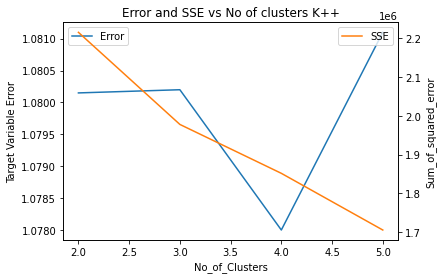
\includegraphics[width=0.5\columnwidth]{hw#4/16.png}
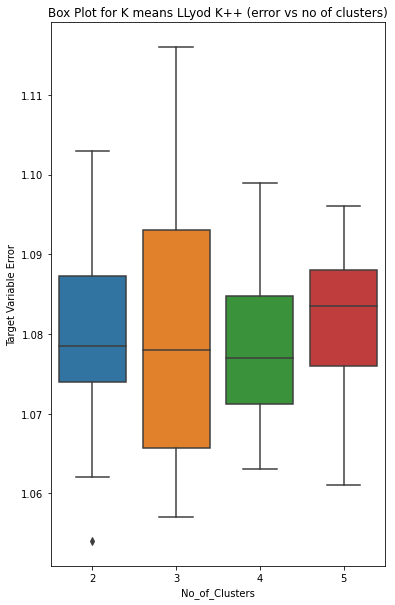
\includegraphics[width=0.5\columnwidth]{hw#4/17.png}
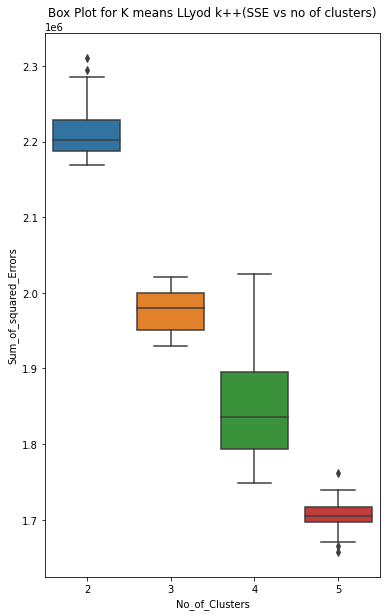
\includegraphics[width=0.5\columnwidth]{hw#4/18.png}
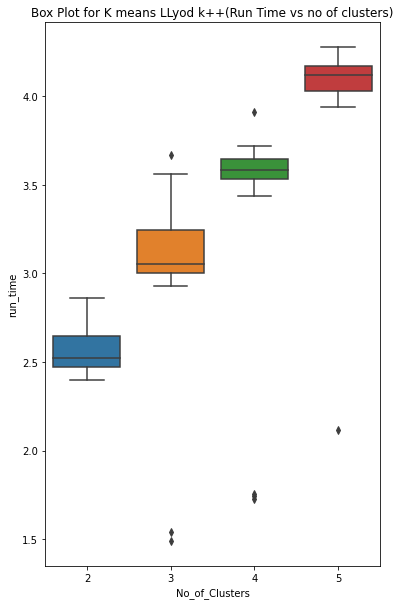
\includegraphics[width=0.5\columnwidth]{hw#4/19.png}
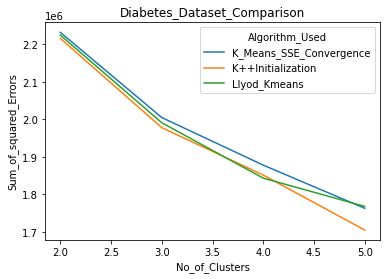
\includegraphics[width=0.5\columnwidth]{hw#4/20.png}
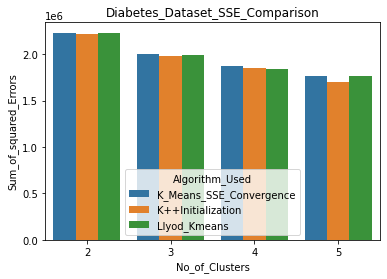
\includegraphics[width=0.5\columnwidth]{hw#4/21.png}
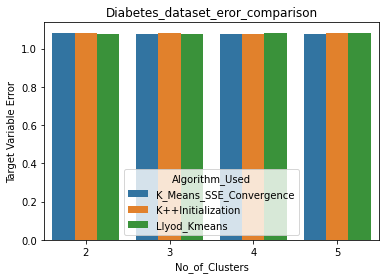
\includegraphics[width=0.5\columnwidth]{hw#4/22.png}

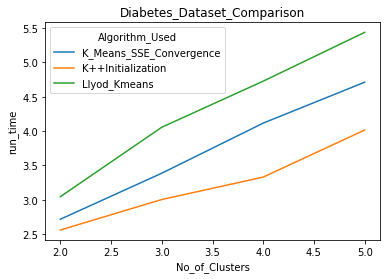
\includegraphics[width=0.5\columnwidth]{hw#4/23.png}
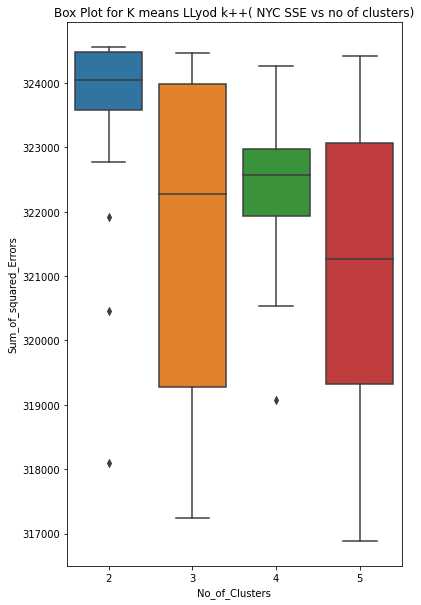
\includegraphics[width=0.5\columnwidth]{hw#4/26.png}
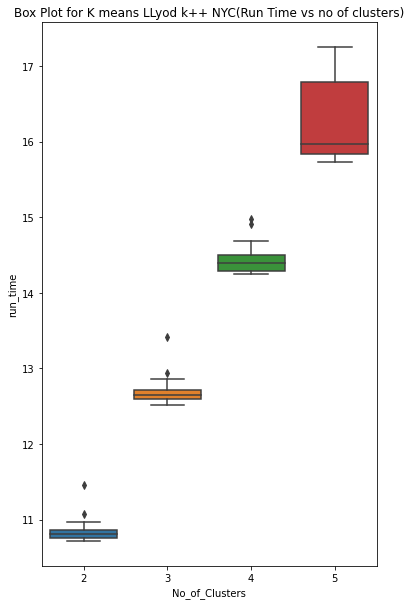
\includegraphics[width=0.5\columnwidth]{hw#4/27.png}
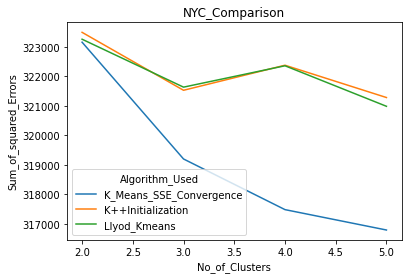
\includegraphics[width=0.5\columnwidth]{hw#4/28.png}
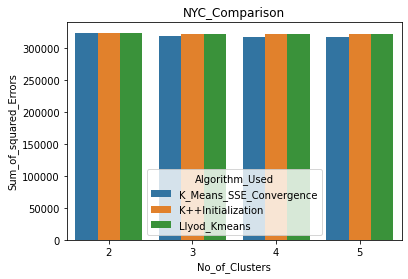
\includegraphics[width=0.5\columnwidth]{hw#4/29.png}
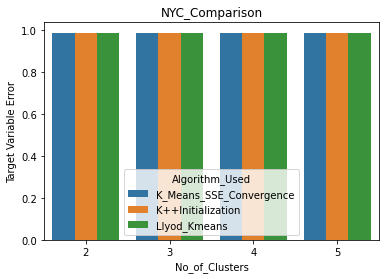
\includegraphics[width=0.5\columnwidth]{hw#4/30.png}
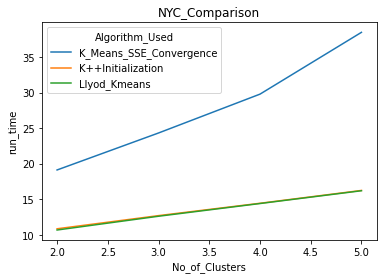
\includegraphics[width=0.5\columnwidth]{hw#4/31.png}
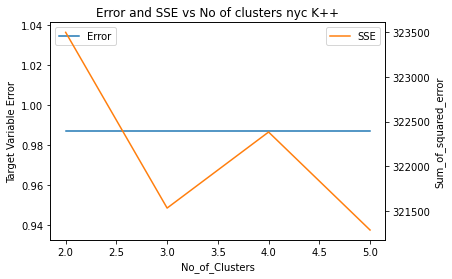
\includegraphics[width=0.5\columnwidth]{hw#4/39_kpp.png}


\end{subfigure}



\subsection{Discussion of Findings}
Answer here$\ldots$
\begin{itemize}
    \item \textbf{Summarisation of Paper for K means}
    item k-means++ is a variation of the k-means clustering 
    algorithm that aims to improve its performance and accuracy 
    by selecting more informative initial seed points.
    \item In standard k-means, the initial seed points are 
    randomly selected, which can result in poor cluster 
    assignments and slow convergence.
    \item k-means++ selects the initial seeds in a way that 
    maximizes the distances between them, ensuring that they 
    are well distributed across the data space.
    \item This approach reduces the likelihood of selecting 
    suboptimal seed points and improves the final clustering 
    quality.
    \item The k-means++ algorithm has been shown to outperform 
    the standard k-means algorithm on a wide range of datasets.
    \item The advantages of k-means++ become more pronounced as 
    the dimensionality of the data increases.
    \item Have implemented K means ++ Initialization and have signiicantly reduced the errors.
    \item For the Diabetes Dataset when error calculagted by K means and error calculated by K means ++ is deduced we get the below error metric
    
\item Cluster        difference

\item 1     9035.03725
\item 2   30161.40420
\item 3   7083.35030
\item 4    71473.21780
\item For the NYC dataset we are getting similar reduction in errors, thus With the Implementation of K means ++ there is a significant reduction in error.

\item Graphs for Diabetes Dataset
\item From the graphs we can conclude that SSE Decreases as the number of cluster increases
\item Also the Target variable after initializing with K means ++ replicates the original classes and thus when we increase the clusters the imbalance is reduced 
\item The box plots indicates the run time of the Algorithm increases as the number of clusters increase
\item The median value of Dataset for SSE decreases when the number of clusters increases.

\item textbf{Comparison Graphs for Diabetes Dataset}
\item When compared the three algorithms we can dedude
\item The sum of Square Errors reduction is highest in K Means ++ Initialization and when we increase the number of clusters K++ Means has the lowest SSE
\item The barplots compare the SSE error between all the algorithms and it clearly indicates that K means ++Initialization has an edge over othe algorithms
\item However when we plot the time the Llyod's K means has high run time, However this can be an anomaly of distance calculations.
\item The general notation suggests as K means calculates the clusters and it has number of iterations higher than regular k means thus it should have high run time

\item \textbf{Graphs for Nyc Dataset}
\item We can conclude even after initializing the clusters from K means ++ the error has decreased
\item This can be shown in the comparison graph
\item From the box plots we can conclude that as the number of clusters increase the run time increases
\item The median SSE also decreases as we increase the number of clusters.

\item \textbf{Comparison for Algorithms NYC}
\item The Sum of Square Errors is decreasing the max in SSE converenge
\item The overall error remains constant as the data is sparse.

\item \textbf{Conclusions}
\item Some factors to consider when deciding whether to use K-means++ initialization:
\item Dataset size: K-means++ initialization is more useful for larger datasets. For smaller datasets, random initialization may work just as well.
\item Clustering performance: If the K-means algorithm is not producing good quality clusters, it may be worth trying K-means++ initialization to see if it improves performane
\item Computational efficiency: K-means++ initialization can be more computationally expensive than random initialization. If you are working with very large datasets or have limited computing resources, random initialization may be a better choice.

\end{itemize}

\end{homeworkProblem}

%----------------------------------------------------------------------------------------
%	PROBLEM 7
%----------------------------------------------------------------------------------------

\begin{homeworkProblem}
 In this question, you are asked to make use of  the  \textit{R/Python} libraries for $k$-means. The elbow technique is used to determine  optimal cluster number.  Find the optimal cluster number for the Diabetes and New York Times Comments data sets using elbow method (for  $2 \leq k \leq 15$). Provide plots that show the total SSE for each $k$. Discuss your results [\textbf{20 points}].

\subsection{R/Python script }
\begin{lstlisting}[language=R]
# Sample R Script With Highlighting

\end{lstlisting}

\begin{lstlisting}[language=Python]
import pandas as pd
import numpy as np
import matplotlib.pyplot as plt
from sklearn.cluster import KMeans
from tqdm import tqdm

# Load data from CSV file
data = df_diabetes_final
columns=df_diabetes_final.columns

#Extract features
X = data[['age', 'admission_type_id', 
'discharge_disposition_id','admission_source_id', 
'time_in_hospital', 'num_lab_procedures','num_procedures', 
'num_medications','number_outpatient','number_emergency', 
        'number_inpatient', 'number_diagnoses','max_glu_serum', 
        'A1Cresult', 'metformin', 'glimepiride', 'glipizide',
       'glyburide', 'pioglitazone', 'rosiglitazone', 'insulin', 
       'change',
       
       'diabetesMed', 'readmitted', 'gender_Female', 
       'gender_Male',
       
       'race_AfricanAmerican', 'race_Asian', 'race_Caucasian', 
       'race_Hispanic',
       'race_Other']]

# Create a list to hold the Sum of Squared Distances (SSD)
ssd = []

# Create KMeans objects for k=1 to k=16
for k in tqdm(range(1, 16)):
    kmeans = KMeans(n_clusters=k, random_state=42)
    kmeans.fit(X)
    ssd.append(kmeans.inertia_)

# Plot elbow curve
plt.plot(range(1,16), ssd)
plt.title('Elbow Curve of Diabetes Dataset')
plt.xlabel('Number of Clusters')
plt.ylabel('SSD')
plt.show()


import pandas as pd
import numpy as np
import matplotlib.pyplot as plt
from sklearn.cluster import KMeans
from tqdm import tqdm

# Load data from CSV file
data = count_vectorizer_df
data=data.fillna(0)

# Create a list to hold the Sum of Squared Distances (SSD)
ssd = []

# Create KMeans objects for k=2 to k=16
for k in tqdm(range(2, 16)):
    kmeans = KMeans(n_clusters=k,random_state=42)
    kmeans.fit(data)
    ssd.append(kmeans.inertia_)

# Plot elbow curve
plt.plot(range(2, 16), ssd)
plt.title('Elbow Curve of New York Dataset')
plt.xlabel('Number of Clusters')
plt.ylabel('SSD')
plt.show()



\end{lstlisting}



\subsection{Plots }
Place images here with suitable captions.
\textbf{Diabetes Dataset}
\begin{subfigure}

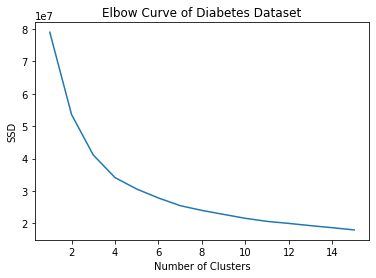
\includegraphics[width=0.5\columnwidth]{hw#4/24.png}
\end{subfigure}

\textbf{New York Comments Dataset}
\begin{subfigure}

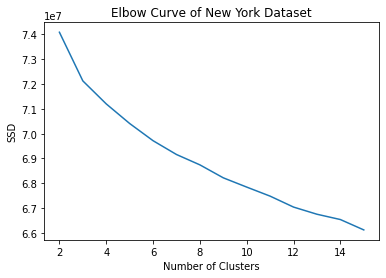
\includegraphics[width=0.5\columnwidth]{hw#4/25.png}
\end{subfigure}
\subsection{Discussion of Findings}
Answer here$\ldots$
\begin{itemize}
    \item From the graph of Elbow of Diabetes dataset there is not a proper value or an elbow in the graph since the error is monotonously decreasing
    \item Visually we can select the clusters from 4 to 6
    \item However we can check that the slope does not change from cluster 10 and hence that could be potential cluster 
    \item However because the curve is not stable we can see we require domain knowledge to guess adequate number of clusters
    \item However there are situations where elbow method provides less information, and we can use other methods like
    \item Silhouette analysis: Silhouette analysis measures how 
    similar an object is to its own cluster compared to other 
    clusters. The silhouette score ranges from -1 to 1, with 
    higher scores indicating that the object is well-matched to 
    its own cluster and poorly matched to neighboring clusters. 
    The optimal k value is the one that maximizes the average silhouette score across all data points.
    \item From the graph of Elbow of New York dataset there is not a proper value or an elbow in the graph since the error is monotonously decreasing
    
    \item Visually we can select the clusters from 10 to 12
    \item However we can check that the slope does not change from cluster 12 and hence that could be potential cluster 
    \item However because the curve is not stable we can see we require domain knowledge to guess adequate number of clusters.
    \item Since the elbow method doesnt work for NYC dataset we can take other measures.
    \item However there are situations where elbow method provides less information, and we can use other methods like
    \item Silhouette analysis: Silhouette analysis measures how 
    similar an object is to its own cluster compared to other 
    clusters. The silhouette score ranges from -1 to 1, with 
    higher scores indicating that the object is well-matched to 
    its own cluster and poorly matched to neighboring clusters. 
    The optimal k value is the one that maximizes the average silhouette score across all data points.
    

\end{itemize}

\end{homeworkProblem}

\newpage
\section*{Extra credit}

This part is optional. 


\begin{enumerate}



\item \href{https://ieeexplore.ieee.org/stamp/stamp.jsp?tp=&arnumber=9139397&tag=1}\kb \ calculates the distance of a data point from the centroid to find the annular region in which the data point resides. The annular region helps determine which neighbor centroids should be included in distance computations.  This improves the run-time over earlier approaches by avoiding expensive computations. Run  your program, $C_{k_{ball}}$, against the Diabetes and New York Times Comments data sets. Report the total error rates for $k = 2,\ldots 5$ for 20 runs each for both data sets. Moreover, compare $C_{k}$, $C_{k_{SSE}}$, $C_{k++}$ and $C_{k_{ball}}$'s run time for $k = 2,\ldots 5$ for 20 runs using both data sets. Presenting the results that are easily understandable.  Plots are generally a good way to convey complex ideas quickly, i.e., box plot.  Discuss  your results  [\textbf{30 points}].\\ 


\subsection{R/Python script }
\begin{lstlisting}[language=R]
# Sample R Script With Highlighting

\end{lstlisting}

\begin{lstlisting}[language=Python]
# Sample Python Script With Highlighting
\end{lstlisting}

\subsection{Discussion of Findings}
Answer here$\ldots$

\subsection{Plots }
Place images here with suitable captions.

\item The student who has the fastest implementation of  all four clustering algorithms  will receive extra 20 points [\textbf{20 points}]. 
\end{enumerate}


\section{Submission}
You must use \LaTeX{} to turn in your assignments. Please submit the following two files via Canvas:
\begin{enumerate}
    \item A .pdf  with the name \texttt{yourname-hw4-everything.pdf} which you will get after compiling your .tex file.
    \item A .zip file with the name \texttt{yourname-hw4.zip} which should contain your .tex, .pdf, codes(.py, .ipynb, .R, or .Rmd), and a README file. The README file should contain information about dependencies and how to run your codes.
\end{enumerate}




\end{document}